\documentclass[12pt,a4paper]{article}
  \usepackage[toc,page]{appendix}
  \usepackage{longtable}
  \usepackage{amsmath}
  \usepackage{booktabs}
  \usepackage{listings} 
  \usepackage{verbatim}
  \usepackage{graphicx}
  \usepackage{tabularx}
  \usepackage{subfig}
  \usepackage{float}
  \usepackage{multirow}
  \usepackage{pdfpages}
  \usepackage{csvsimple}
  \usepackage{hyperref}
  \usepackage[a4paper,bindingoffset=0.2in,left=0.6in,right=0.6in,top=1in,bottom=1in,footskip=.25in]{geometry}

  \usepackage{listings}
  \usepackage{color}
  \definecolor{white}{rgb}{0.95,0.95,0.95}
  \definecolor{darkgray}{rgb}{.1,.1,.1}
  \definecolor{purple}{rgb}{0.65, 0.12, 0.82}
  \definecolor{green}{rgb}{0,0.6,0}
  \definecolor{gray}{rgb}{0.5,0.5,0.5}
  \definecolor{main}{rgb}{0.06,0.34,0.41}

  \lstdefinelanguage{JavaScript}{
    keywords={typeof, new, true, false, catch, function, return, null, catch, switch, var, if, in, while, do, else, case, break},
    keywordstyle=\color{main}\bfseries,
    ndkeywords={class, export, boolean, throw, implements, import, this, from, default, it, renderer, create, expect, toMatchSnapshot, const, let, toEqual, simulate, shallow, find, exists, toBeTruthy, describe},
    ndkeywordstyle=\color{main}\bfseries,
    identifierstyle=\color{black},
    sensitive=false,
    comment=[l]{//},
    morecomment=[s]{/*}{*/},
    commentstyle=\color{purple}\ttfamily,
    stringstyle=\color{red}\ttfamily,
    morestring=[b]',
    morestring=[b]"
  }

  \lstset{
    language=JavaScript,
    backgroundcolor=\color{white},   % choose the background color
    basicstyle=\footnotesize,        % size of fonts used for the code
    breaklines=true,                 % automatic line breaking only at whitespace
    captionpos=b,                    % sets the caption-position to bottom
    commentstyle=\color{green},      % comment style
    escapeinside={\%*}{*)},          % if you want to add LaTeX within your code
    keywordstyle=\color{blue},       % keyword style
    stringstyle=\color{darkgray},     % string literal style
  }

  \hypersetup{%
    pdfborder = {0 0 0}
  }

  \begin{document}
    \begin{titlepage}
      \centering
      {\scshape\LARGE Goldsmiths, University of London \par}
      \vspace{1cm}
      {\scshape\Large Software project final report\par}
      \vspace{1.5cm}
      {\huge\bfseries iLost\par}
      \vspace{2cm}
      {\Large\itshape 
        Ahmed, Muhammad\\
        Chowdhury, Thairan\\
        Davies Minta, Dylan\\     
        Fakrul, Mahmudul\\    
        Farkhani, Hussein\\ 
        Jheng-Hao, Lin\\
        Pecorella, Mariano\\ \par}
      \vfill
      supervised by\par
      \textsc{Tim Blackwell} 
      \vfill
      % Bottom of the page
      {\large \today \par}
    \end{titlepage}
    \tableofcontents
    \newpage
    \section{Introduction}
      \paragraph{} Losing belongings is a common problem, roughly £70 worth of items are lost in public each year. \textsuperscript{[1]} We conducted a survey about lost items to find out if we could create a useful application based on this concern. Following our survey, this statement was found to relate to university students as 89\% of our participants claimed to be susceptible to losing items. This information motivated us to reduce the loss of personal belongings; leading to the development of an item tracking application and a portable tracking device. Our app aims to circumvent the loss of bags and valuables. The user will attach the portable tracker to their bag, allowing it to be tracked using our app. The app will notify the user when the distance between the app and tracker reaches 30m.

      This report will cover five main categories:

      \begin{itemize}
        \item {Development Record}
          We explain the methodology used by our group to decide the technology with which to implement the app’s functionality and the development methods we used. We also describe the way that the development was handled by the team and provide a reflection on its efficiency.

        \item {Formative Evaluation}
          This section of the report describes our assessment with users during development. The formative evaluation details what we did during user testing and its outcomes.

        \item { Design and Implementation }
          An overview of our final design and implementation, including any changes from our initial ideas with justifications for the significant decisions we made.

        \item { Quality Assurance}
          We detail our approach to Quality Assurance and the testing carried out, including our results. An assessment of how well our final system imitates our initial requirements with Justifications of any changes we made to the requirements.

        \item { Summative Evaluation}
          A descriptive evaluation of the methods, results and conclusions of our final software.
      \end{itemize}

    \section{Development Record}
      \subsection{Teams} 
        % 400 - 500 words
        \paragraph{}During in the implementation stage, we set up an organisation {\bf GSoft} on GitHub and we were divided into three teams, {\bf iOS app}, {\bf Android app} and {\bf Backend/Tracker team}, which shows in figure \ref{fig:Development Teams}. Each team was grouped by 2 to 3 people who were more interested in that topic or technology. Some of us were interested in more than two areas then he would join two of the teams. The list of the team members can be found in table \ref{table:Teams}. 
        \begin{figure}[H]
          \centering
          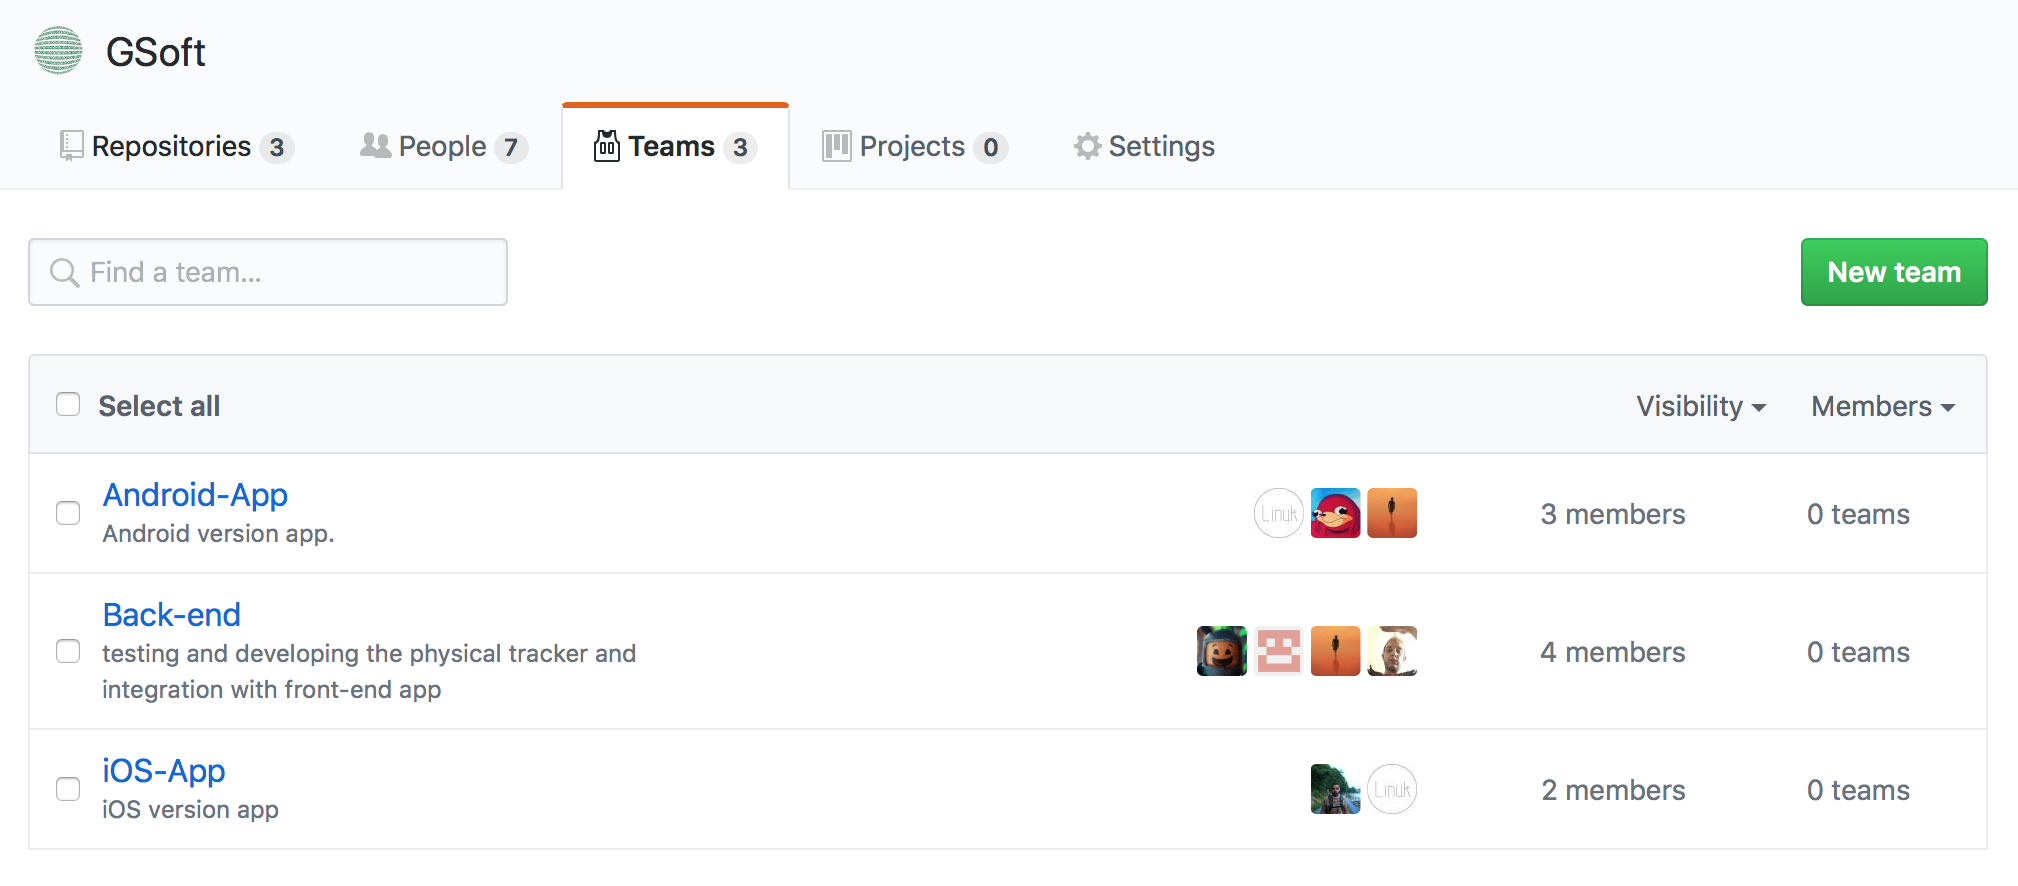
\includegraphics[width=1\textwidth]{../assets/development-records-teams.png}
          \caption{Development Teams on Github}
          \label{fig:Development Teams}
        \end{figure}

        \begin{table}[H]
          \centering
            \begin{tabularx}{\textwidth}{l X}
              \hline
               Team & Members \\ \hline
               iOS app & Jheng-Hao(leader), Muhammad \\
               Android app & Dyland(leader), Mahmudul, Jheng-Hao \\ 
               Backend/Tracker  & Hussein(leader), Thairan, Mahmudul, Mariano \\
              \hline
            \end{tabularx}
            \caption[Table caption text]{Teams}
            \label{table:Teams}
        \end{table}        

      \subsection{Technology Selection} 

        \paragraph{}Development TeamsEach team was responsible for how and what technology to use as long as the production could be made on time. We believed this methodology had these advantages in terms of the limited development time:

        \begin{itemize}
          \item {React Agilely}: Compare to have a poll with all members of our group, it was agiler to come to the decision within 2 or 3 people within one team. Since each team could react to the situation and resolve the issues in a more efficient way.
          \item {Specialities differ}: Our group was divided by our interests and specialities, we trusted each team could make the best decision for the whole team with their research and experience. For example, the iOS app team would not interfere how tracker team implemented the physical components at all, and how Android app was implemented would not be the backend/tracker team's concern. All teams were trusted that they would make the best decisions.
        \end{itemize}
        
        \paragraph{}Even though the team was separated, it was important to keep everyone on the same page. So each technological decision or propose was documented as an architecture decision record(ADR), which enabled us to have an overview of all the technological changes. According to Michael Nygard, each ADR contains five columns\cite{ArchitectureDecisionRecord}: 

        \begin{itemize}
          \item Title: A brief description of the propose.
          \item Context: {\bf Why} do we need to make the decision or change.                   
          \item Decision: {\bf What} is the response toward the decision.
          \item Status: current status of the decision which, should be {\bf accepted}, {\bf rejected} or {\bf deprecated}.
          \item Consequences: {\bf What} become better or worse because of the decision.
        \end{itemize}

        Please find more, complete architecture decision records in \ref{appendix:Architecture Decision Records}.
        
        To keep the whole group has the latest information, We used several channels on Slack to keep everyone updated. Such as the {\bf iOS channel} was the place containing all updates related to iOS application development, which shows in figure \ref{fig:Slack iOS Channel}. 
        
        \begin{figure}[H]
          \centering
          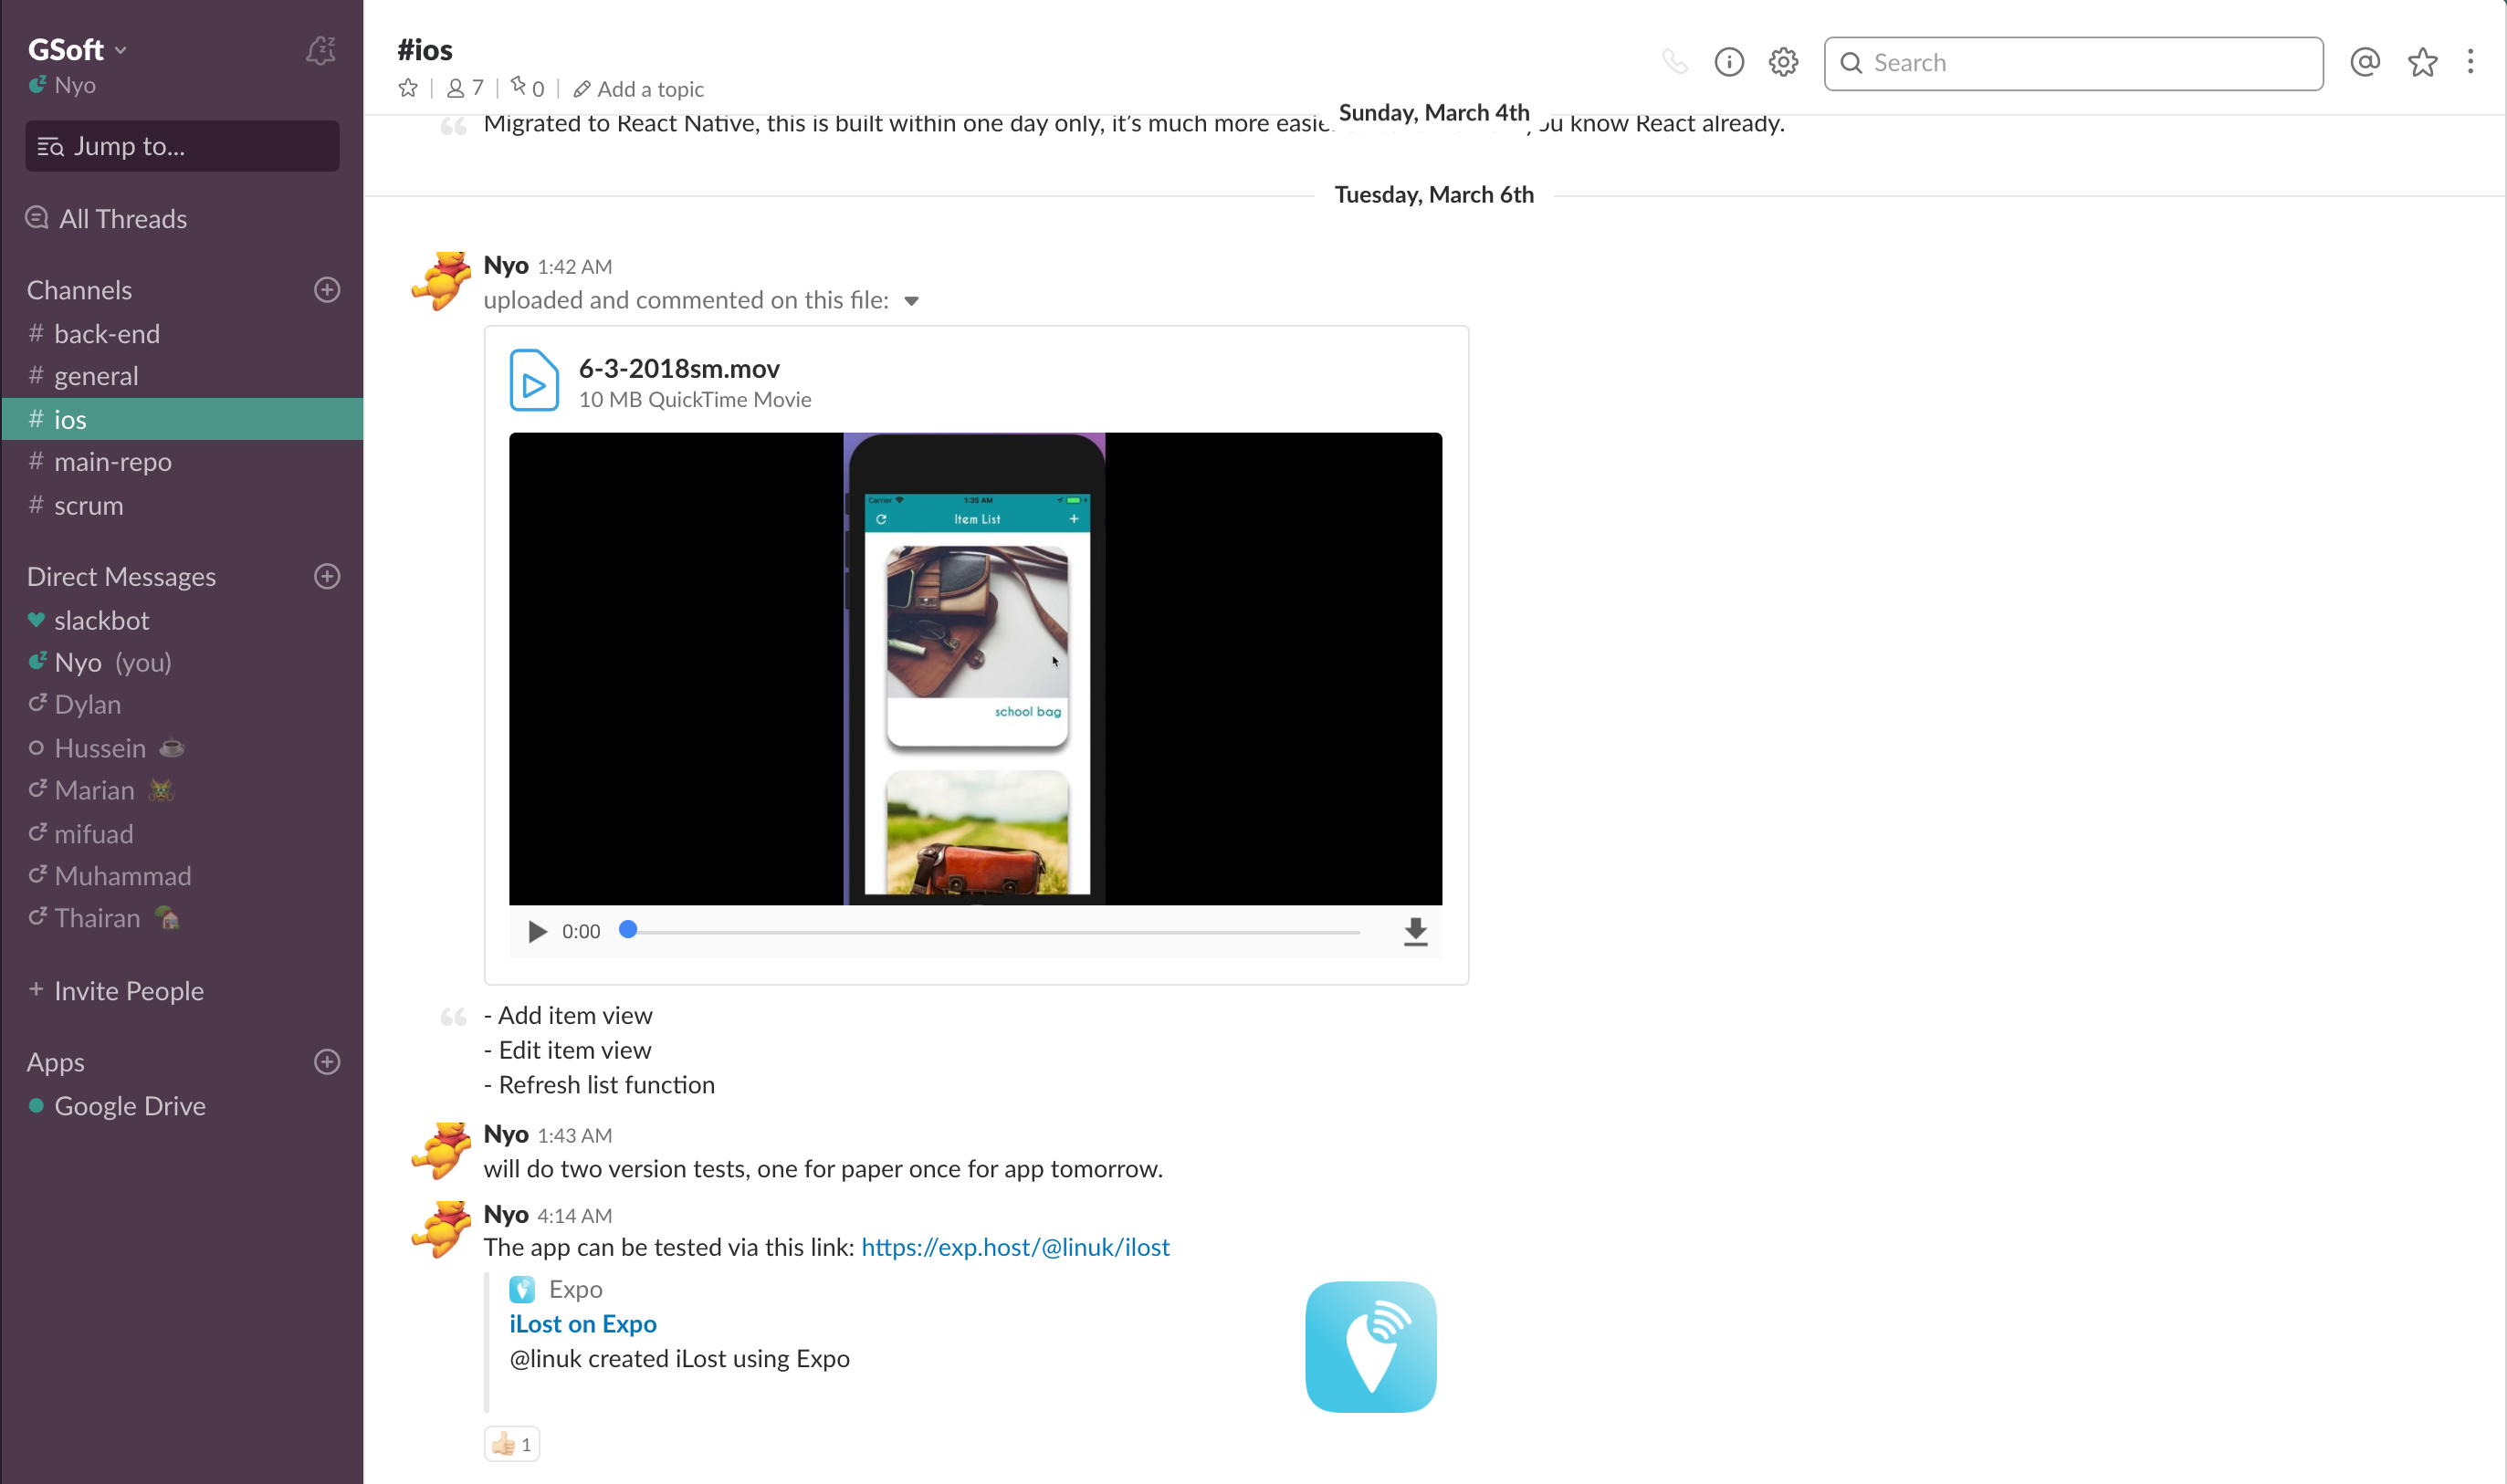
\includegraphics[width=1\textwidth]{../assets/development-records-slack-ios-channel.png}
          \caption{Slack iOS Channel}
          \label{fig:Slack iOS Channel}
        \end{figure}

      \subsection{Agile Development} 
        
        \paragraph{}Our team tried out two agile development methodologies, {\bf Scrum} and {\bf Kanban}.

        \subsubsection{Scrum Development}
          \paragraph{}Since we could not actually devote all of our time to develop the application, it would not be reasonable to do the daily scrum and have a meeting day-to-day for all of us. So in the beginning, we tried to set up a routine to simulate the daily scrum with Slack.

          \paragraph{}We defined 3 days as one sprint and whenever a sprint was finished, the team needed to answer three questions in the Scrum channel on Slack:
          
          \begin{itemize}
            \item What did I complete last time that contributed to the team meeting our sprint goal?
            \item What do I plan to complete this time to contribute to the team meeting our sprint goal?
            \item Do I see any impediment that could prevent the team or me from meeting our sprint goal?
          \end{itemize}    

          \paragraph{}Unfortunately, not every team could follow the sprint process and make any progress every three days. Sometimes a team might work for a sprint then stopped for two sprints since other modules might have a deadline or coursework. Hence, this scrum process was not actually conducted properly and stopped after few weeks after started. The example records show in figure \ref{fig:Slack Scrum Channel}. 

          \begin{figure}[H]
            \centering
            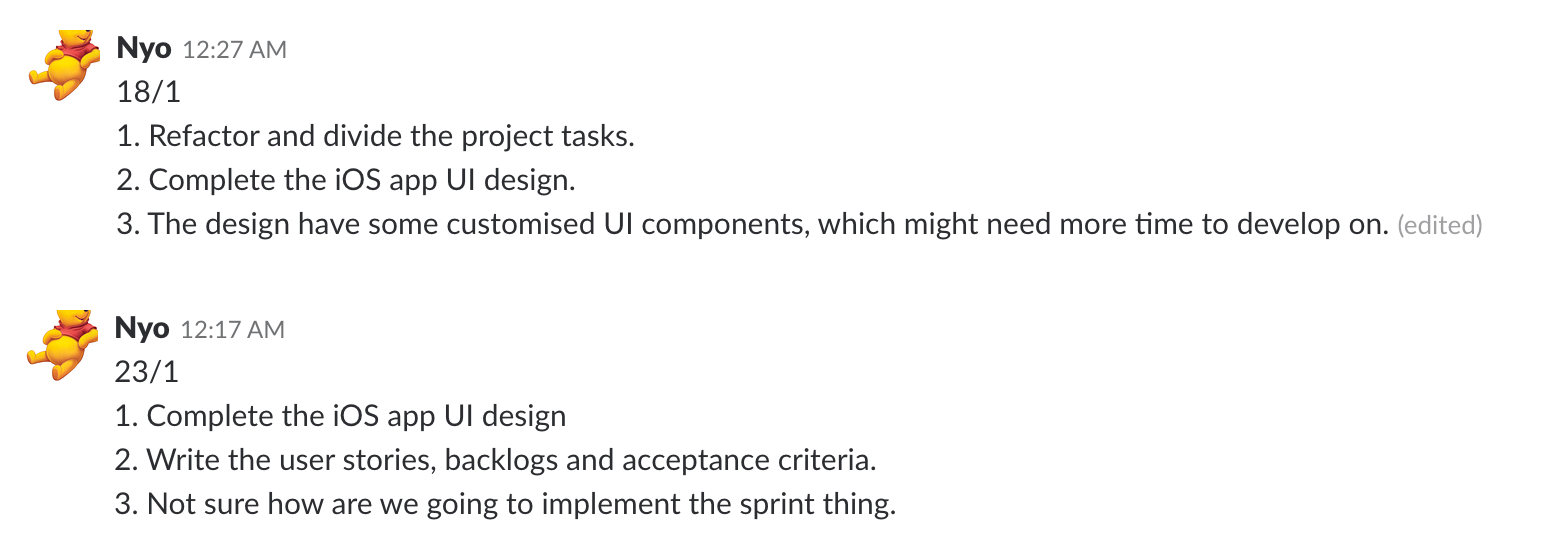
\includegraphics[width=1\textwidth]{../assets/development-records-slack-scrum-channel.png}
            \caption{Slack Scrum Channel}
            \label{fig:Slack Scrum Channel}
          \end{figure}
          
          \paragraph{}At the middle of the development stage, our supervisor suggested us to meet 2 hours a day and 2 to 4 days a week, work and team and engage the team building, since the progress tracking form showed that the working hours were really unbalanced and some people apparently did not put enough effort into the project. 
          
          \paragraph{}We made a daily sprint schedule, shows in figure \ref{fig:Daily Sprint} and followed the time to do work together. Everyone should follow the schedule and spend at least two days a week to work together as a team. It went well and most of us were able to follow the schedule. We worked in RHB306a, 35 Cafe or the Whitehead building lab. But since the strike started, the daily sprint stopped again because not all of us were coming to the campus due to the long distance between home and the university. 

          \begin{figure}[H]
            \centering
            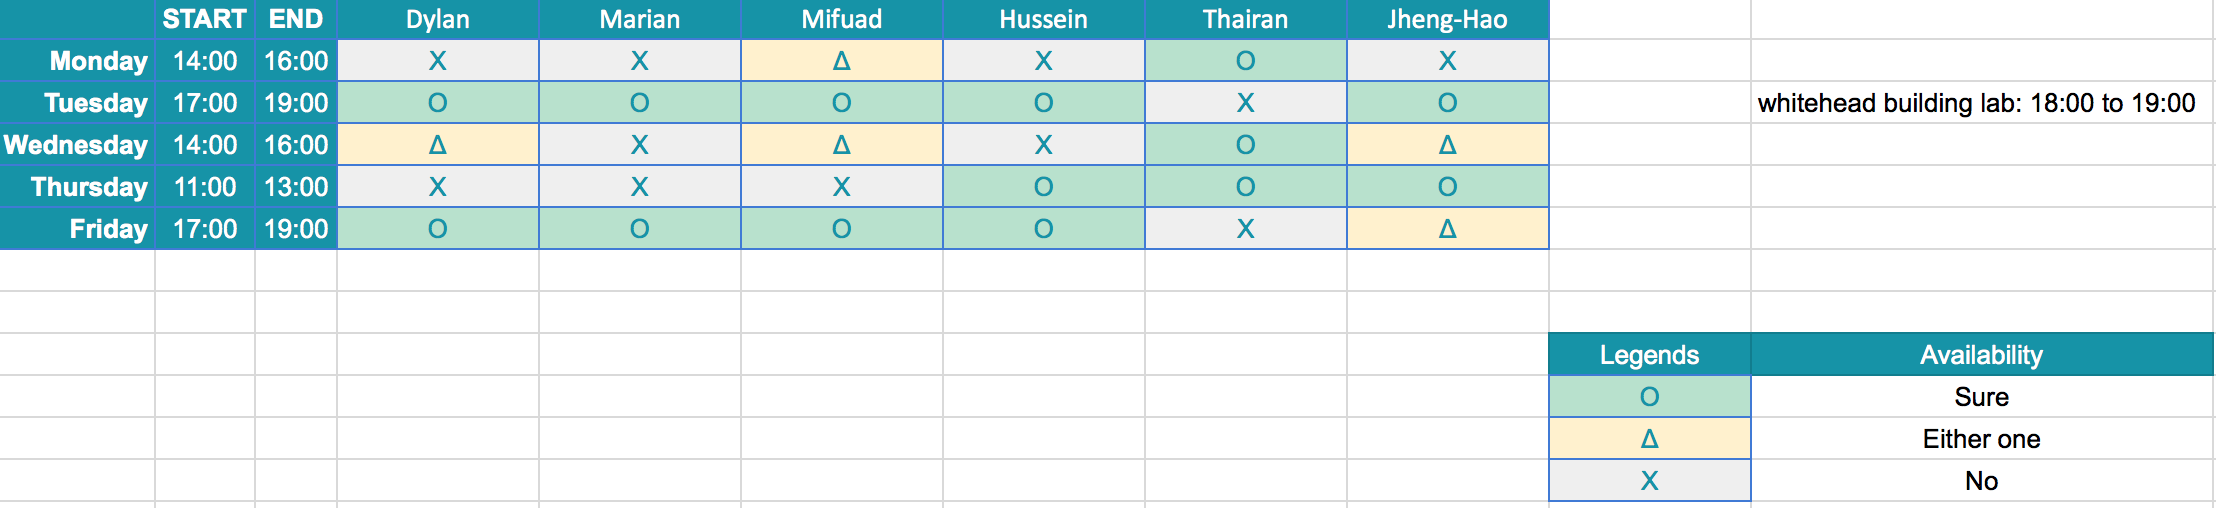
\includegraphics[width=1\textwidth]{../assets/development-records-daily-sprint.png}
            \caption{Daily Sprint}
            \label{fig:Daily Sprint}
          \end{figure}

        \subsubsection{Kanban}
          \paragraph{}Apart from the Scrum, Kanban was also implemented with the backlogs in our development to demonstrate the development progress. We tried to keep our project management tool simple and easy to approach, so we not only used GitHub for version control but also for the project feature, which we used it as the Kanban. The iOS  development kanban was shown in \ref{fig:iOS Development Kanban}.

          \begin{figure}[H]
            \centering
            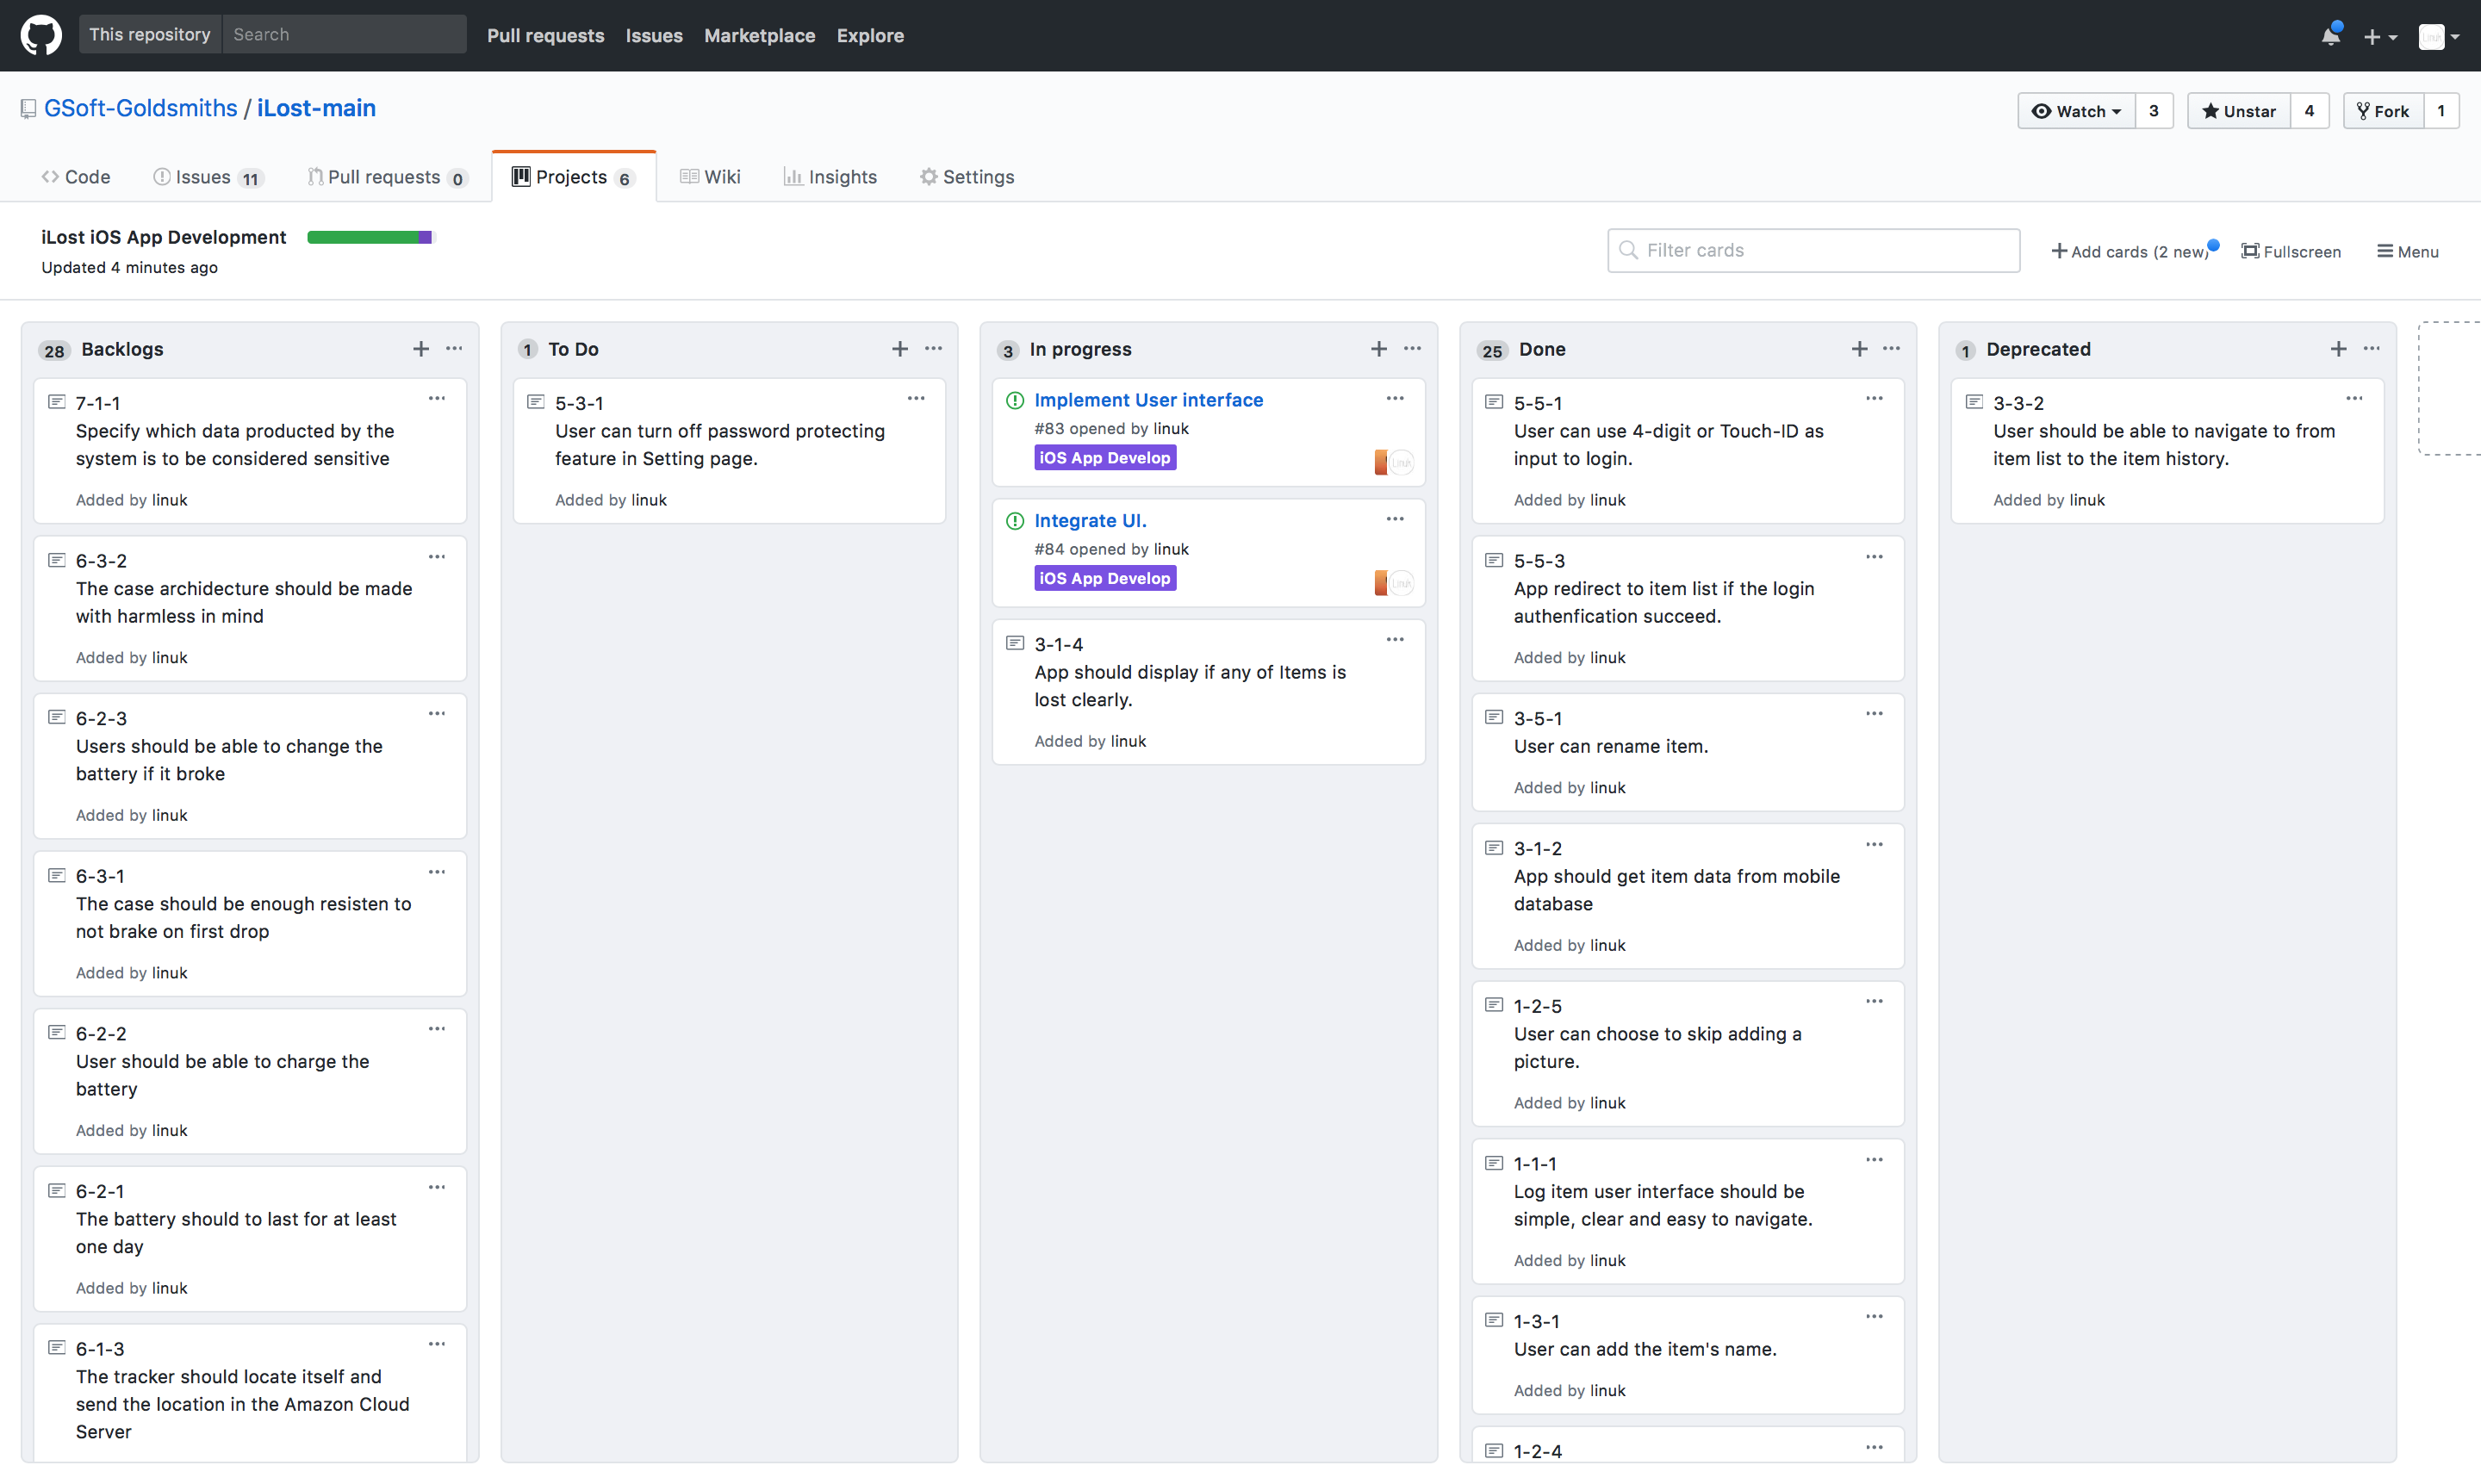
\includegraphics[width=1\textwidth]{../assets/development-records-ios-kanban.png}
            \caption{iOS app Kanban}
            \label{fig:iOS Development Kanban}
          \end{figure}
         
          Our kanban contained five columns which shows in Table \ref{table:Kanban Columns}:
          
          \begin{table}[H]
            \centering
              \begin{tabularx}{\textwidth}{l X}
                \hline
                Column & Description  \\ \hline
                Backlogs & The task is scheduled to be develop, but it is possible to be assigned deprecated if it is no longer needed. \\ 
                To Do & The task is going to be develop.  \\ 
                In Progress & The task is currently developing.  \\ 
                Done & The task has been completed.   \\ 
                Deprecated & The task no longer needs to be developed.\\                  
                \hline
              \end{tabularx}
              \caption[Table caption text]{Kanban Columns}
              \label{table:Kanban Columns}
          \end{table}
          
          Apart from the normal columns: To Do, In Progress and Done, we also added {\bf Deprecated} to store the features or tasks did not fit the needs anymore. Kanban gave a nice and clean overview of the current developing process, especially for people from other teams.
        
        \subsubsection{Behavior Driven Development}
          \paragraph{}In order to produce the minimum viable product(MVP), we followed the Behavior Driven Development(BDD) to develop our product. To implement this methodology, we wrote the backlogs of requirements specification at the beginning of the development stage. These requirements provided us with an overview of what was more urgent in what stage. 

          \paragraph{}For example, displaying the item's position and historical locations was one of the most important functionality, so its' priority was {\bf Must} and needed to be finished at the {\bf MVP} stage. On the other hand, navigating to the item by triggering Google Map was helpful but might take longer to develop, so the priority was {\bf Should} and it should be developed at the {\bf Final} stage. 
          
          \paragraph{}Here was our development process of BDD:
          
          \paragraph{1. Requirements specification}Review the backlogs and pick one from them to work on based on the priority and the estimated development time. Please can find the details of the backlogs in section \ref{section:Development Process - Backlogs}, Development Process - Backlogs.
          
          \paragraph{2. Design}Review the how was the data storage, data flow and the user interface design, then design how should this requirement be fulfilled. Such as displaying the item list in the item list view, we would need to implement two view components, an item list cell view and an item list table view. The item's properties data, including items id, name and photo, would be stored in the table view's state and the list cell would receive the props from the table view and render the item's properties.
          
          \paragraph{3. Development}Put the design into actual codes.
          
          \paragraph{4. Integration}Integrate the new view component with previously developed view components. Such as connecting the item list view with the item details view, where users could see its' location with a map.
          
          \paragraph{5. QA reviews}Conduct the quality assurance of the functionalities of latest and previously developed components. Please find more details in the chapter \ref{chapter:Quality Assurance}, Quality Assurance.
          
          \paragraph{6. Usability tests}After several developments, we would bundle them as a new version of our mobile application. Then do the usability tests to test if any of the components, user interface or user experience could be improved. Please find more details in the chapter \ref{Chapter:Formative Evaluation}, Formative Evaluation.
          
          \paragraph{7. Maintance}After the usability tests, we did some improvement based on the usability testing results. 
          
          \paragraph{}This was a cycle process, after step 7 we went back to step 1 and kept going.

      \subsection{Development Process}
        \subsubsection{Backlogs}
          \label{section:Development Process - Backlogs}
          \paragraph{}Based on the user stories we made in the proposal, not only did we added more but also wrote sub-user stories and acceptance criteria for each of them. We had a list contain backlogs stored in Google SpreadSheet, which contained these columns: 

          \begin{table}[H]
            \centering
              \begin{tabularx}{\textwidth}{l X}
                \hline
                Column & Description  \\ \hline
                User Story ID & The user story ID or sub-user story ID, a user story ID should be 1, 2, 3...n, and sub-user story should be 1-1, 1-2, 1-3, ... 1-m  where 1 is the parent user story.\\ 
                User Story & A brief description of the user story, starting with "As a user I want to ..." to describe what is the users' needs. Then followed by "so that ..." to explain why users need it. \\ 
                Backlog ID & An ID number for the backlog, a sub-user story may contain more than one backlog to satisfy the sub-user story. If a sub-user story ID is  3-5, then the task ID will be 3-5-1, 3-5-2, 3-5-3, ... 3-5-p.  \\ 
                Acceptance Criteria & A description of the backlog which describe how the mobile application or the tracker would satisfy the user stories. \\ 
                Priority & The priority of this backlog, should be {\bf Muse}, {\bf Should} or {\bf Could}. \\                  
                Dev Days & The estimated developing times in days, 8 hours counted as one day. \\                  
                Phase & In which phase should the backlog be finished, in our case was {\bf MVP} or {\bf Final}. \\                  
                Process & The current developing process, which should be {\bf ToDo}, {\bf In Progress}, {\bf Deprecated} or {\bf Done}.  \\                  
                \hline
              \end{tabularx}
              \caption[Table caption text]{Backlogs Columns}
              \label{table:Backlogs Column}
          \end{table}
          
          For example, the user story 3, {\bf Track Item: User uses App to see the tracking list and track Item.} This section has 7 sub-user stories, which shows in table \ref{table:Backlog Example: User Story 3}: 
          
          \begin{table}[H]
            \centering
              \begin{tabularx}{\textwidth}{l X}
                \hline
                 User Story ID & User Story \\ \hline
                 3-1 & As a user, I want to view the tracking item list so that I can view my item and look up more detail if I want. \\
                 3-2 & As a user, I want to activate or deactivate tracker so that I can save my mobile and the tracker's batteries. \\
                 3-3 & As a user, I want to see the location history in a map format of the item so that I can track/look for it if it's lost. \\
                 3-4 & As a user, I want to navigate me to my item so that find it quicker. \\
                 3-5 & As a user, I want to edit my item detail so that I can change the tracking item. \\
                 3-6 & As a user, I want to delete the item so that I can stop tracking the item for good. \\
                \hline
              \end{tabularx}
              \caption[Table caption text]{Backlog Example: User Story 3}
              \label{table:Backlog Example: User Story 3}
          \end{table}   
          
          Take sub-user story 3-1 as an example. In order to satisfy this user story, we had 4 backlogs and acceptance criteria to meet the requirements. Each of them had their own priority, estimated development days, phase and process. So this backlog will look like figure \ref{fig:Backlog Example: Sub-user story 3-1}:
          
          \begin{figure}[H]
            \centering
            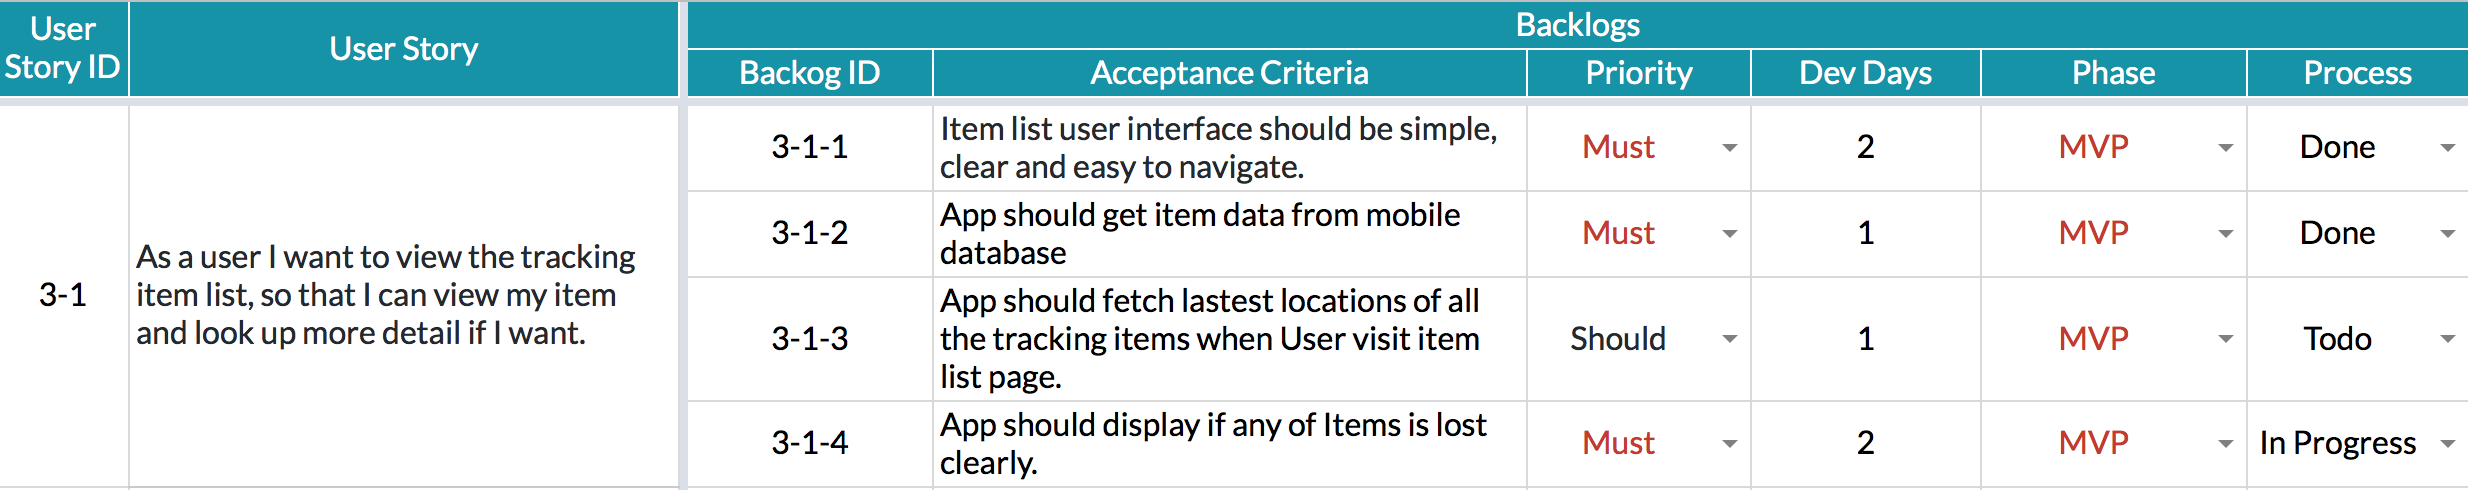
\includegraphics[width=1\textwidth]{../assets/development-records-backlog-example.png}
            \caption{Backlog Example: Sub-user story 3-1}
            \label{fig:Backlog Example: Sub-user story 3-1}
          \end{figure}
          
          The full backlogs can be found in the appendix \ref{appendix:backlogs} and it was used to create our kanban showed in figure \ref{fig:iOS Development Kanban}, which kept the developing process recorded easily to follow.        
          
        \subsubsection{Progress Tracking}
          \paragraph{}To record our progress, we kept using the same progress tracking form as the last term, and this term we did some improvement:

          \begin{itemize}
            \item {Lock every week}: To prevent any team members from modifying the resource hours dishonestly, a range of the form was locked every week. Only records within recent two weeks were allowed to be added. 
            \item {Status documented in more detail}: To increase the traceability and convincing evidence, each resource hours commitment was asked to provide a more detailed description. Instead of {\it reporting writing}, it was improved to be {\it Final report: Formative Evaluation - mobile application test}.
          \end{itemize}

          Please find the full progress tracking form in appendix \ref{appendix:progress-tracking-form}.\\
          
          Until March 16, the total working time during these two terms is {\bf 581.9 hours}. All these hours contribution includes all lab sessions, supervisor meetings, daily sprint and self-independent working time. 58.7\% was contributed by Hussein and Jheng-Hao as shown in figure \ref{fig:Progress Tracking Diagram}. The top contributor is Jheng-Hao with 222.95 hours contributed, while the last is Chin with 26.5 hours recorded. The line chart displays that the commitment became dramatically different since the start of the second term. Most of the team members stopped to work in the second term, excluding Hussein and Jheng-Hao who still kept working continuously.
          
          \begin{figure}[H]
            \centering
            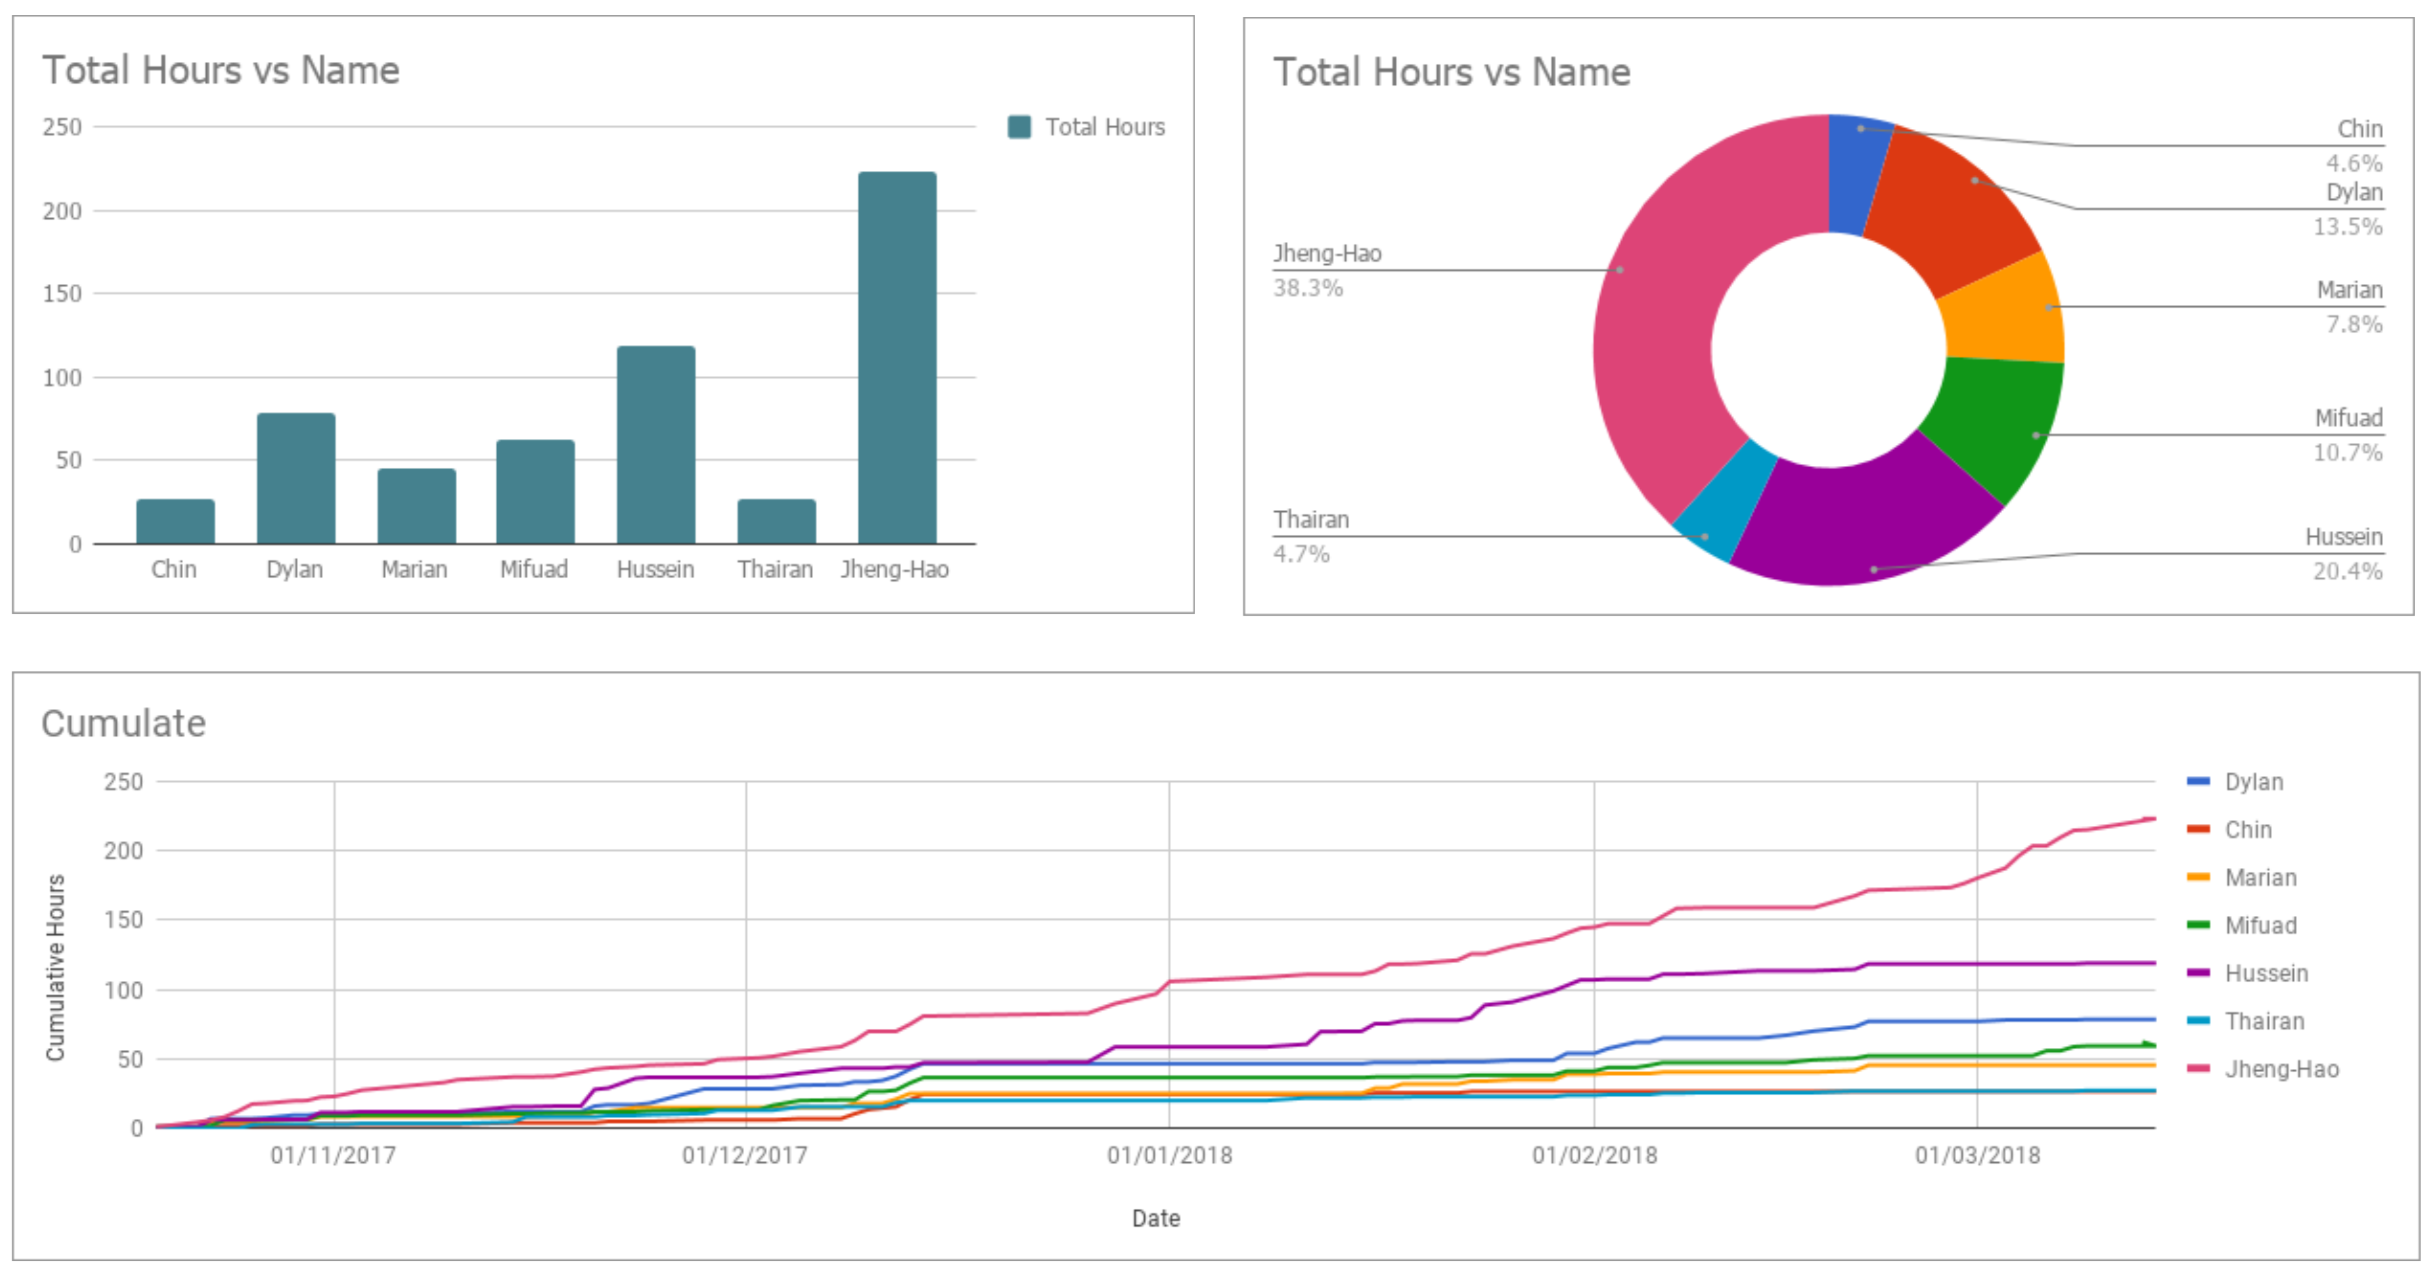
\includegraphics[width=1\textwidth]{../assets/development-records-progress-tracking-diagram.png}
            \caption{Progress Tracking Diagram (until March 16th)}
            \label{fig:Progress Tracking Diagram}
          \end{figure}

      \subsubsection{Evaluation}

        \paragraph{Scrum} This methodology is suitable for a team where they tend to work together in a fixed time, day-to-day. Even though we had scheduled the daily sprint time, not everyone would attend since it was not compulsory and registered. Only few sprint sessions at the beginning went well. In terms of time management, not every one of us were able to contribute fixed time every one or two days, so we could not have a daily sprint or even weekly sprint. Unless we have could work full time for this project and everyone is willing to meet at a place and work together, or it would be better not to implement Scrum in our team. 
        
        \paragraph{Kanban} Regards of project management, Kanban went well, but it would be better if we could have a workspace where we could combine our backlogs and Kanban. We found that there are two web applications that could provide this kind of services: Clubhouse and Jira They are the web applications where we can add user stories which link to kanbans at the same time. It would be nice to use this kind of tools to save time if the team has enough budget.
        
        \paragraph{Backlogs} The backlogs were the most important things we could improve on. We only listed the basic cases while the extreme use stories were not in our backlogs. For example, {\bf "As a user I want my tracker to keep working in the snowing seasons"} could be in our user story as our product should still be functional in the winter season.

        \paragraph{Progress Tracking} In terms of progressing tracking form, it should added one column which links to the contributions, either their GitHub commit or documentation. It was not be nice to record n hours working without any evidence but it did happen. Also, it was not really feasible to use working hours to represent the contributions. With the same task, people spend less time to finish the same job should be rewarded higher compared to who spend longer period to do so. But we were not able to do this since everyone worked on different tasks. It would be fairer if each task could be evaluated by the importance, whoever completes the higher importance means contributing more. We should have a contribution list which records everyone's participation. Then with the list, we could write the peer access form in a more objective point of view.

    \section{Formative Evaluation}
      \label{Chapter:Formative Evaluation}
      % total 1650 words
      \subsection{iOS App Evaluation} 
        
          % total 1000 words
        \subsubsection{Objectives and Questions}
          % 100 words
          \paragraph{}
            We wrote quantitative tasks to test the usability of our mobile application\cite{WritingTasks}. The purpose of the tests was to test if the participants can actually finish the task with the application, and we could learn from the process to observe how users used our application and improve it if any issue or confusion was raised. 

            \begin{figure}[H]
              \centering
              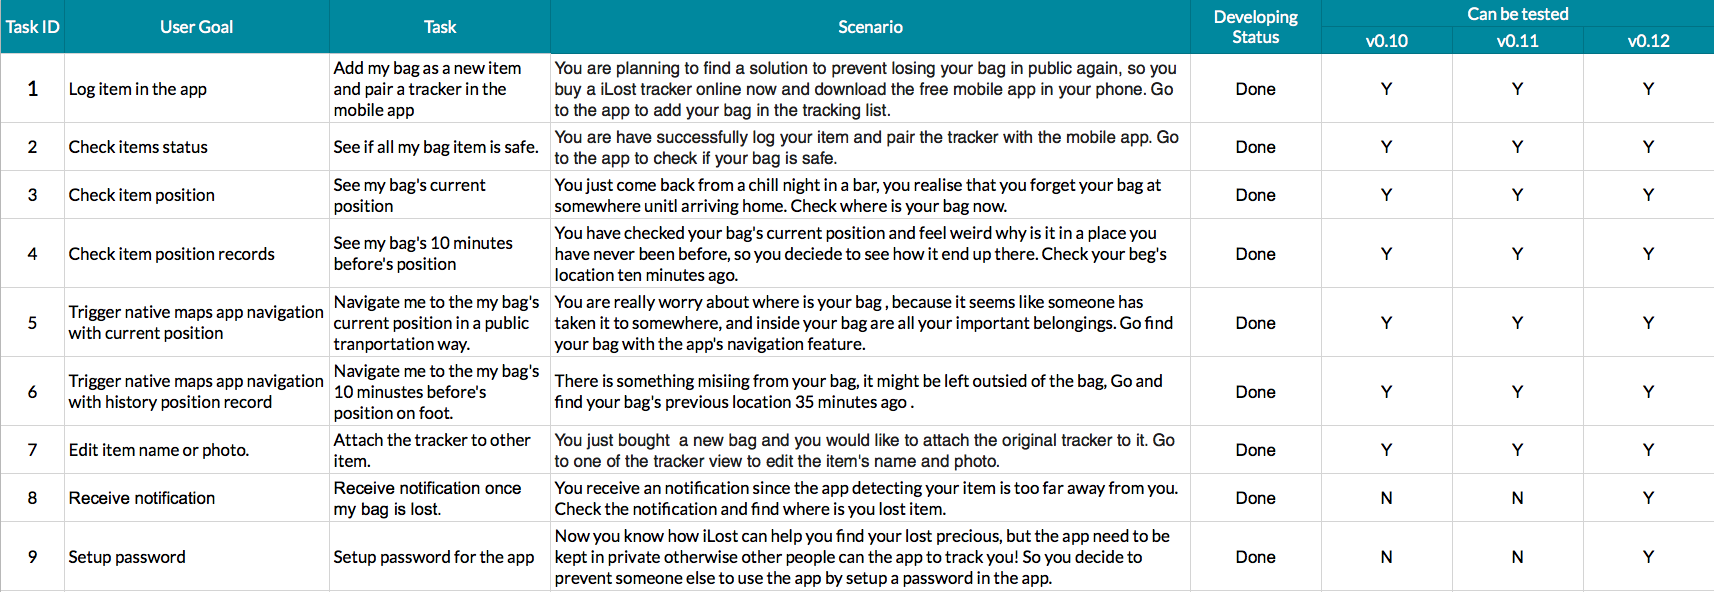
\includegraphics[width=1\textwidth]{../assets/usability-test-task-list.png}
              \caption{Usability test task list}
              \label{fig:Usability test task list}
            \end{figure}

            \begin{table}[H]
              \centering
                \begin{tabularx}{\textwidth}{l X}
                  \hline
                  Column & Description  \\ \hline
                  Task ID & Identify the number of the task.  \\ 
                  User Goal & What is the objective we need users to perform.  \\ 
                  Task & The process in terms of completing the goal.  \\ 
                  Scenario & A setup scenario for engaging testers to use the application in a real-life case.   \\ 
                  Developing Status & Current latest developing status of the functionality of this task, it should be {\bf To do}, {\bf In Progress} and {\bf Done}.\\ 
                  Can be tested &  Whether the functionality of the application is ready to be tested in each version.\\ 
                  \hline
                \end{tabularx}
                \caption[Table caption text]{Usability test task list columns}
                \label{table:Usability test task list columns}
            \end{table}

            Figure \ref{fig:Usability test task list} demonstrates our tasks and goals. Table \ref{table:Usability test task list columns} shows what the columns stand for.

        \subsubsection{Participants, Location and Setup}
          % 100 words
          \paragraph{} According to Jakob Nielsen, testing 5 users in a usability study could find almost as many usability problems as testing more participants\cite{HowManyTestUsers}. Following this theory, our application was tested with 5 participants for each version. The study was taken place in the library of the Goldsmiths, University of London, and the participants were the students who used to bring a bag to the campus daily. Totally we have conducted three versions of the application.
          
        \subsubsection{Methodology and Measures}
          % 100 words
          \paragraph{} Firstly, we explained what was our project about and asked participants to sign up the consent form which can be found in appendices \ref{appendix:consent-form}. During the test, the participants were provided an iPhone with the application built-in to test. An observer would guide them through the tasks and the scenarios, then took notes of how the participants reacted to the application. For each task, the observer would record it was successfully completed or failed. The records would help us to build the success rates diagram which helped us to understand which usability needed to be improved\cite{SuccessRates}. 
        
        \subsubsection{Evaluation}
          
          \begin{figure}[H]
            \centering
            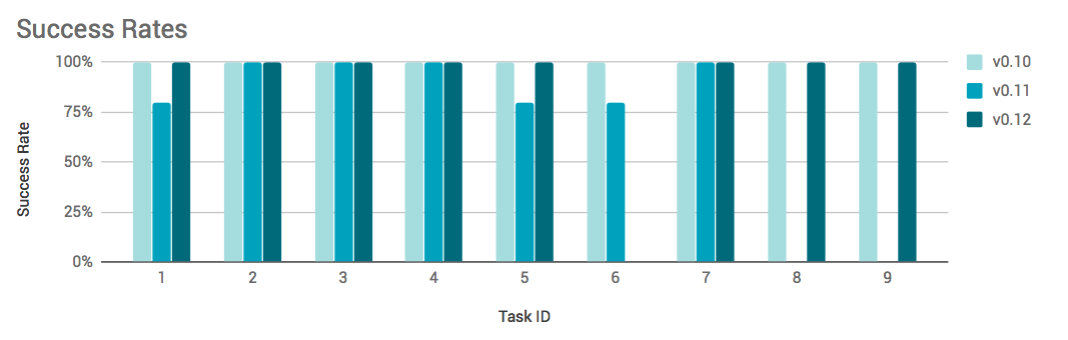
\includegraphics[width=1\textwidth]{../assets/usability-test-success-rates.png}
            \caption{iOS App Success Rates Diagram}
            \label{fig:iOS App Success Rates Diagram}
          \end{figure}

          \paragraph{v0.10} The tested subject was the application prototype built in {\bf Adobe XD}, which was one of the best design tools to test the prototype. Thanks to the well-designed user interfaces, the goals were easy to achieved and all the tasks were all succeeded. The result could only prove that the user interfaces guided the users to the right view, but it could not actually reflect on the usability of the real application. After all, Adobe XD could only let users walk through each view by clicking, while an actual iOS application should support swipe or other gestures. It was more like a paper prototype usability test.
          
          \paragraph{v0.11} We benefited most from this test since this test was the native mobile application we where the participants can actually use it like other application. This version was built in React Native and tested in Expo which a tool and service which we used to build the mobile native application with React Native. During this test, we received several comments towards the {\bf add item view}. For example, the camera icon in that view was originally used as a button. But some of the users could not really regard it as a button but a decoration since it was colourful. Also, the placeholder of the item name field was {\bf Item Name} instead of a prompt message which confused some of the participants as well. So after this test, we resolved the issues and the difference shows in figure \ref{fig:usability-test-ios-v010-improvements}. The task 8 and 9 were not developed completely at the moment so there was not any record.

          \begin{figure}[H]
            \centering
            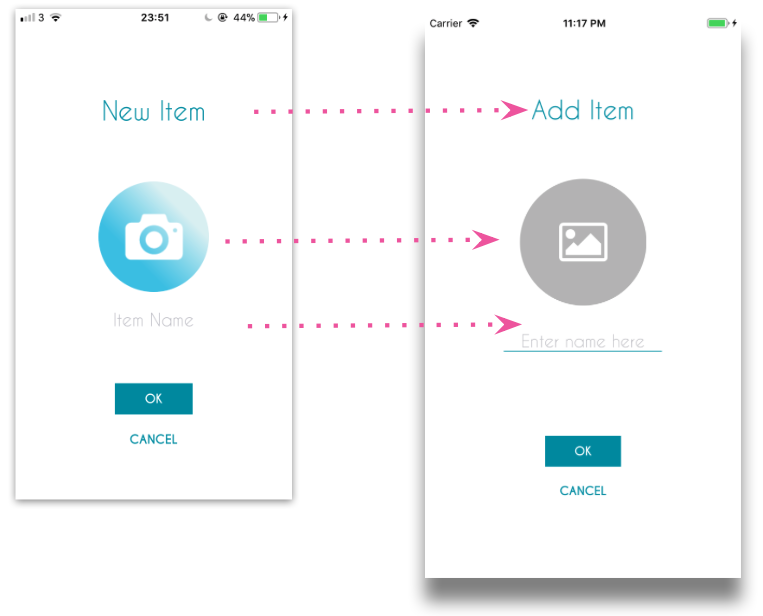
\includegraphics[width=0.7\textwidth]{../assets/usability-test-ios-v010-improvements.png}
            \caption{Improvement of the add item view}
            \label{fig:usability-test-ios-v010-improvements}
          \end{figure}

          \paragraph{v0.12} After the previous test, we not only improved some of the user interfaces but also removed some of the features. It is worth notice that there is no record of task 6, which is {\bf navigating to previous locations of the item's location history}. The reason we removed this task was that this goal was not really helpful. The participants commented that it was not beneficial to navigate to the previous locations, they cared about the current location of the item more. So thanks to the feedback, we removed task 6 and eliminated the functionality of navigating through history locations which made the application more simple. 
        
        \subsection{Tracker Evaluation}
            total 700 words
          \subsubsection{Objectives and Questions}
            100 words
          \subsubsection{Location, Setup and Participants}
            100 words
          \subsubsection{Methodology and Measures}
            100 words
          \subsubsection{Tracker v0.10 Evaluation}
            150 max words
          \subsubsection{Tracker v0.11 Evaluation}
            150 max words
        \subsection{Conclusion}
          % 200 max words
          Even though the tasks could be completed, but in terms of the user experience, we still had space to improved. 
      \newpage
    \section{Design and Implementation}
    \section{Quality Assurance} % 1600 - 2000 words
      \label{chapter:Quality Assurance}
      
      \subsection{Process} % 100 words
        \paragraph{} We conducted two types of quality assurance to ensure our mobile application working as we expected, including black-box testing and white-box testing. While the white-box testing focused on the functionalities, such as how an item list view should react when an add new item button was clicked, the black-box testing covered how a view component or a function should be rendered or implemented, such as a button should render a text on it based on what text state passed to it. Usually, the black-box tests were conducted after the white-box tests, since the functionalities could be functional only if the component worked properly. 

        \paragraph{} Since the time limitation, only the iOS version was fully tested, but the test cases could be implemented in both version of the application.

      \subsection{Black-box Tests}
        \subsubsection{Method and Environment} % 150 words
          \paragraph{} The black-box tests covered the functional testing testing of the use scenarios, they were developed by the acceptance criteria of the backlogs. Since our mobile application was not really complicated and complex, we did not implement any automated way to conduct the tests but manually merely. We chose {\bf use case testing} as our approach to conduct the static tests, since it was the quickest way we could conduct the tests with existing resources.
          
          \paragraph{} The iOS application was written in React Native, it was imported and tested in the Expo \cite{Expo} application on an iPhone 6. Expo is a mobile application where everyone can download others' React Native codes and run on their iPhone or iPad, rather than paying USD 3000/year to subscribe the Apple Developer Programme to use TestFlight \cite{TestFlight}, which is the official testing application owned by Apple Inc. 
        
        \subsubsection{Unit Tests} % 500 words
          \paragraph{}Our use cases table was adapted from the format wrote by a software consultant company IntexSoft \cite{UseCaseTestingReference}. The test cases contained the columns shows in table \ref{table:Black-box Test Cases Columns}: 

          \begin{table}[H]
            \centering
              \begin{tabularx}{\textwidth}{l X}
                \hline
                Column & Description  \\ \hline
                ID & Unique ID of the test case \\ 
                Name & Name of the test case.  \\ 
                Goal & The detail description of the purpose of the test goal. \\ 
                Precondition & What need to be satisfied before the test case can be tested.\\
                Success End Condition & The definition of how the test case considered as passed \\
                Feiled End Condition & The definition of how the test case considered as failed \\
                Trigger & How this use scenario is triggered.\\
                Normal Flow & The flow of this test case, such as how the stakeholders react with applicatoin.\\
                Alternative Flows & The details of alternative ways to different successful ends.\\
                Frequency of Use & How often has this uses cases been triggered, we use {\bf Rare}, {\bf Normal} and {\bf Often} to represent various level of the frequency since we did not have a proper statics for each use case.\\
                Assumptions & Any assumptions that were made during the analysis of the use case. \\
                \hline
              \end{tabularx}
              \caption[Table caption text]{Black-box Test Cases Columns}
              \label{table:Black-box Test Cases Columns}
          \end{table}

          \paragraph{} So for example, one of the test cases is to trigger the Apple map and navigate the user to the item's location. The fields look like table \ref{table:Black-box Test Case: Trigger Apple Map}:

          \begin{table}[H]
            \centering
              \begin{tabularx}{\textwidth}{l X}
                \hline
                Column & Description  \\ \hline
                ID & 30 \\
                Name &  Item details view: trigger Apple Map. \\
                Goal &  The application should be able to use the item's location data, pass it to the Apple Map application, and trigger the navigation function and lead the user to the item's location       \\
                Precondition & User is in the item details view.        \\
                Success End Condition & The Apple Map application is triggered after the user taps the navigate button. It gets into the navigation mode and leads the user to the location based on the distance. If the user is closed to the item, then it will navigate the user to the item in "walking" mode. If the item is far from the user it will be in the "transit" mode         \\
                Failed End Condition & The Apple Map application is not triggered after the navigate button is tapped. Or the Apple Map application is triggered but it does not receive the correct location data of the item and activate the navigate mode either.           \\
                Trigger & User taps the navigate button \\
                Normal Flow & 1. The user taps the navigate button. 2. The application triggers the Apple Map application and passes the geolocation of the item to it. 3. Apple Map automatically activates navigation mode and lead the user to the item. \\
                Alternative Flows & N/A \\
                Frequency of Use & Often \\
                Assumptions & There are item's location data stored in the application already \\
                \hline
              \end{tabularx}
              \caption[Table caption text]{Black-box Test Case: Trigger Apple Map}
              \label{table:Black-box Test Case: Trigger Apple Map}
          \end{table}

          \paragraph{} Please find more details of the black-box test cases in the appendix \ref{appendix:black-box-test-cases}

      \subsection{White-Box Tests}
        % 800 words
        \subsubsection{Method and Environment} % 250 words
          \paragraph{}The iOS application was developed in a component-based way, and we tested most of the elements whenever a new one was built. In React Native, there are two types of components, pure components and containers. Pure components do not store any data but render whatever data are passed to them only, The passed data in React are called "props". On the other hand, containers are the components store the data, which is named "state", and render the pure components. In an MVC model, the pure components are more the {\bf View} and the containers are the {\bf Controller}. We were only able to test the pure components at the time limitation. Testing the pure components was relatively easy and quick, and it helped us to debug and boost the developing efficiency.
          
          \paragraph{}The testing framework we chose was Jest\cite{Jest} and Enzyme\cite{Enzyme}, a JavaScript testing framework developed by Facebook. The main reason we chose Jest rather than other testing frameworks was that it was maintained by the same company of React Native. There were not only resourceful community supports but also the official documents were really well documents. These reasons made it one of the trendy testing framework in the React ecosystem. Mocha, another popular JavaScript unit testing framework, was considered too. However, since the iOS team did not have any previous experience with it, so to meet the deadline we chose to use the most familiar tool.
        
          \paragraph{}The iOS application was developed in a component-based way, and we tested most of the elements whenever a new one was built. In React Native, there are two types of components, pure components and containers. Pure components do not store any data but render whatever data are passed to them only, The passed data in React are called "props". On the other hand, containers are the components store the data, which is named "state", and render the pure components. In an MVC model, the pure components are more the {\bf View} and the containers are the {\bf Controller}.
          
          \paragraph{}We were only able to test the pure components at the time limitation. Testing the pure components was relatively easy and quick, and it helped us to debug and boost the developing efficiency.

        \subsubsection{Test Cases} % 550 word
          \paragraph{}The testing framework we chose were Jest\cite{Jest} and \cite{Enzyme}, Jest was a JavaScript testing framework developed by Facebook and Enzyme was the React component testing utility. There were several reasons made us choose these tools rather than other testing frameworks. Firstly, Jest and Enzyme were developed and maintained by Facebook and Airbnb developers team. The resourceful community supports and the well-written official documents were all really helpful. These reasons made these tools became the trendy testing frameworks in the React ecosystem. Mocha, another popular JavaScript unit testing framework, was considered too. However, the iOS team did not have any previous experience with it, so we chose to use the most familiar tools in order to meet the deadline.
          
          \paragraph{}Jest and Enzyme were combined together into one testing file and test if a component was rendered properly. Button was one of the pure components which has been unit-tested, which contained two props: {\bf text} and {\bf handler}. The {\bf text} was the text rendered on the button, and the {\bf handler} was the function which would be called whenever the button was pressed. The button code shows in Listing \ref{lst:Button.jsx}:
        
          \begin{lstlisting}[caption=Button.jsx, label={lst:Button.jsx}]

      import React from 'react';
      import { mainFontBold, style } from '../styles/variables';
      import { Text, TouchableHighlight } from 'react-native';

      export default ({ text, handler }) => (
        <TouchableHighlight
          style={style.button}
          onPress={() => handler()}
        >
          <Text style={{ color: '#fff', fontFamily: mainFontBold }}>{text}</Text>
        </TouchableHighlight>
      );

          \end{lstlisting}
        
          In terms of the button component, we tested it in four aspects: 
          \begin{itemize}
            \setlength\itemsep{0em}
            \item{\bf Rendered without crashing}: We used the snapshot API from Jest. A snapshot was JSON string of the component, during the test the newly built component would be converted to JSON and compared with the previously built snapshot. The test would be passed if both snapshots were the same.  
            \item{\bf Rendered with correct elements}: Text and TouchableHighlight should be rendered in the button component, we tested if they existed.
            \item{\bf Rendered with correct props}: The text field was rendered with a text prop, which should be rendered in the Text component inside. So we tested it if the Text component was rendered with the correct text.
            \item{\bf The button handler should work if the button is pressed}: Tested if the handler was functional if the button was pressed simulated.
          \end{itemize} 

          The actual code shows in Listing \ref{lst:Button.test.jsx}:
          \begin{lstlisting}[caption=Button.test.jsx, label={lst:Button.test.jsx}]
      
      import React from 'react';
      import { Text, TouchableHighlight } from 'react-native';
      import { shallow, configure } from 'enzyme';
      import renderer from 'react-test-renderer';
      import Adapter from 'enzyme-adapter-react-16';

      import Button from '../../src/components/Button';

      configure({ adapter: new Adapter() });

      describe('<Button />', ()=>{
        it('renders without crashing', () => {
          const rendered = renderer.create(<Button text="title" handler={() => {}}/>).
            toJSON();
          expect(rendered).toMatchSnapshot();
        });
        
        it('renders with correct elements', () => {
          const wrapper = shallow(<Button text="title" handler={() => {}}/>);
          expect(wrapper.find(Text).exists()).toBeTruthy();
          expect(wrapper.find(TouchableHighlight).exists()).toBeTruthy();
        });

        it('renders with correct props', () => {
          const wrapper = shallow(<Button text="title" handler={() => { testData =  "button is pressed"; }}/>);
          const text = wrapper.find(Text);
          expect(text.props().children).toEqual("title");
        });

        it('the button handler should work if the button is pressed', () => {
          let testData = "before button is pressed";
          const wrapper = shallow(<Button text="title" handler={() => { testData =  "button is pressed"; }}/>);
          wrapper.find(TouchableHighlight).simulate('press');
          expect(testData).toEqual("button is pressed");
        });
      });

          \end{lstlisting}

          \paragraph{} This is how we unit test the pure components. Our application used most of the native components provided by Expo SDK and React Native, so only 4 components were needed to be tested: {\bf Button}, {\bf FullPageView}, {\bf ItemListCell} and {\bf PasswordInput}. The other 9 container components were tested if they were rendered properly without crashing only. The source code for unit testing could be found in our public Github repository: \url{https://github.com/GSoft-Goldsmiths/iLost-main/tree/master/src/react-native-app/tests}


      \subsection{Evaluations} % 200 words
        \paragraph{} Both types of tests helped us to maintain the quality of our software before actually conducting the usability tests with the participants, and here are some points could be improved in terms of our quality control:
        \begin{itemize}
          \item {\bf Add extreme cases}: The test cases aimed to test the normal use cases since we did not have much time to test the extreme cases. But in real life, the boundary value analysis is relatively important in terms of the software testing as well apart from the normal use cases.
          \item {\bf Automated the tests}: During the black-box tests we conducted the tests manually, but in fact, we could automate the process and save us a lot of time. In fact, Jest, the tool we used to automated unit testing, supports the automated application testing, it is worthy to do more research on it.
          \item {\bf More tests related to the tracker}: Since the limited time, we did not have much time left to do the tests for the physical tracker. It is important to test any part of our product, especially the integration between the tracker and the mobile application should be well tested.
          \item {\bf Follow Test Driven Development(TDD)}: TDD was one of the development methodologies we intended to implement since it controlled the code quality. But the trade off was slowing down the developing speed. For building an MVP, TDD might not be a good option, but in the future development, it would be essential.
        \end{itemize}
       
    \section{Summative Evaluation}
    
    \begin{thebibliography}{20}
      \bibitem{ArchitectureDecisionRecord} M. Nygard, "Blog | Documenting Architecture Decisions | Relevance", Thinkrelevance.com, 2011. [Online]. Available: http://thinkrelevance.com/blog/2011/11/15/documenting-architecture-decisions. [Accessed: 15- Mar- 2018].
      \bibitem{HowManyTestUsers} "How Many Test Users in a Usability Study?", Nielsen Norman Group, 2012. [Online]. Available: https://www.nngroup.com/articles/how-many-test-users/. [Accessed: 01- Mar- 2018].
      \bibitem{WritingTasks} "Writing Tasks for Quantitative and Qualitative Usability Studies", Nielsen Norman Group, 2018. [Online]. Available: https://www.nngroup.com/articles/test-tasks-quant-qualitative/. [Accessed: 14- Mar- 2018].
      \bibitem{SuccessRates} "Success Rate: The Simplest Usability Metric", Nielsen Norman Group, 2001. [Online]. Available: https://www.nngroup.com/articles/success-rate-the-simplest-usability-metric/. [Accessed: 14- Mar- 2018].
      \bibitem{Expo} "Expo", Expo, 2018. [Online]. Available: https://expo.io/. [Accessed: 18- Mar- 2018].
      \bibitem{TestFlight} "TestFlight - Apple Developer", Developer.apple.com, 2018. [Online]. Available: https://developer.apple.com/testflight/. [Accessed: 18- Mar- 2018].
      \bibitem{UseCaseTestingReference} "use case testing - IntexSoft", Intexsoft.com, 2015. [Online]. Available: http://www.intexsoft.com/blog/item/117-use-case-testing.html. [Accessed: 18- Mar- 2018].
      \bibitem{Jest} "Jest · 🃏 Delightful JavaScript Testing", Facebook.github.io, 2018. [Online]. Available: https://facebook.github.io/jest/. [Accessed: 18- Mar- 2018].
      \bibitem{Enzyme} "Introduction · Enzyme", Airbnb.io, 2018. [Online]. Available: http://airbnb.io/enzyme/. [Accessed: 19- Mar- 2018].
    \end{thebibliography}
    
    \begin{appendices}                  
      \section{Development Records}
        \subsection{Backlogs}\label{appendix:backlogs}
          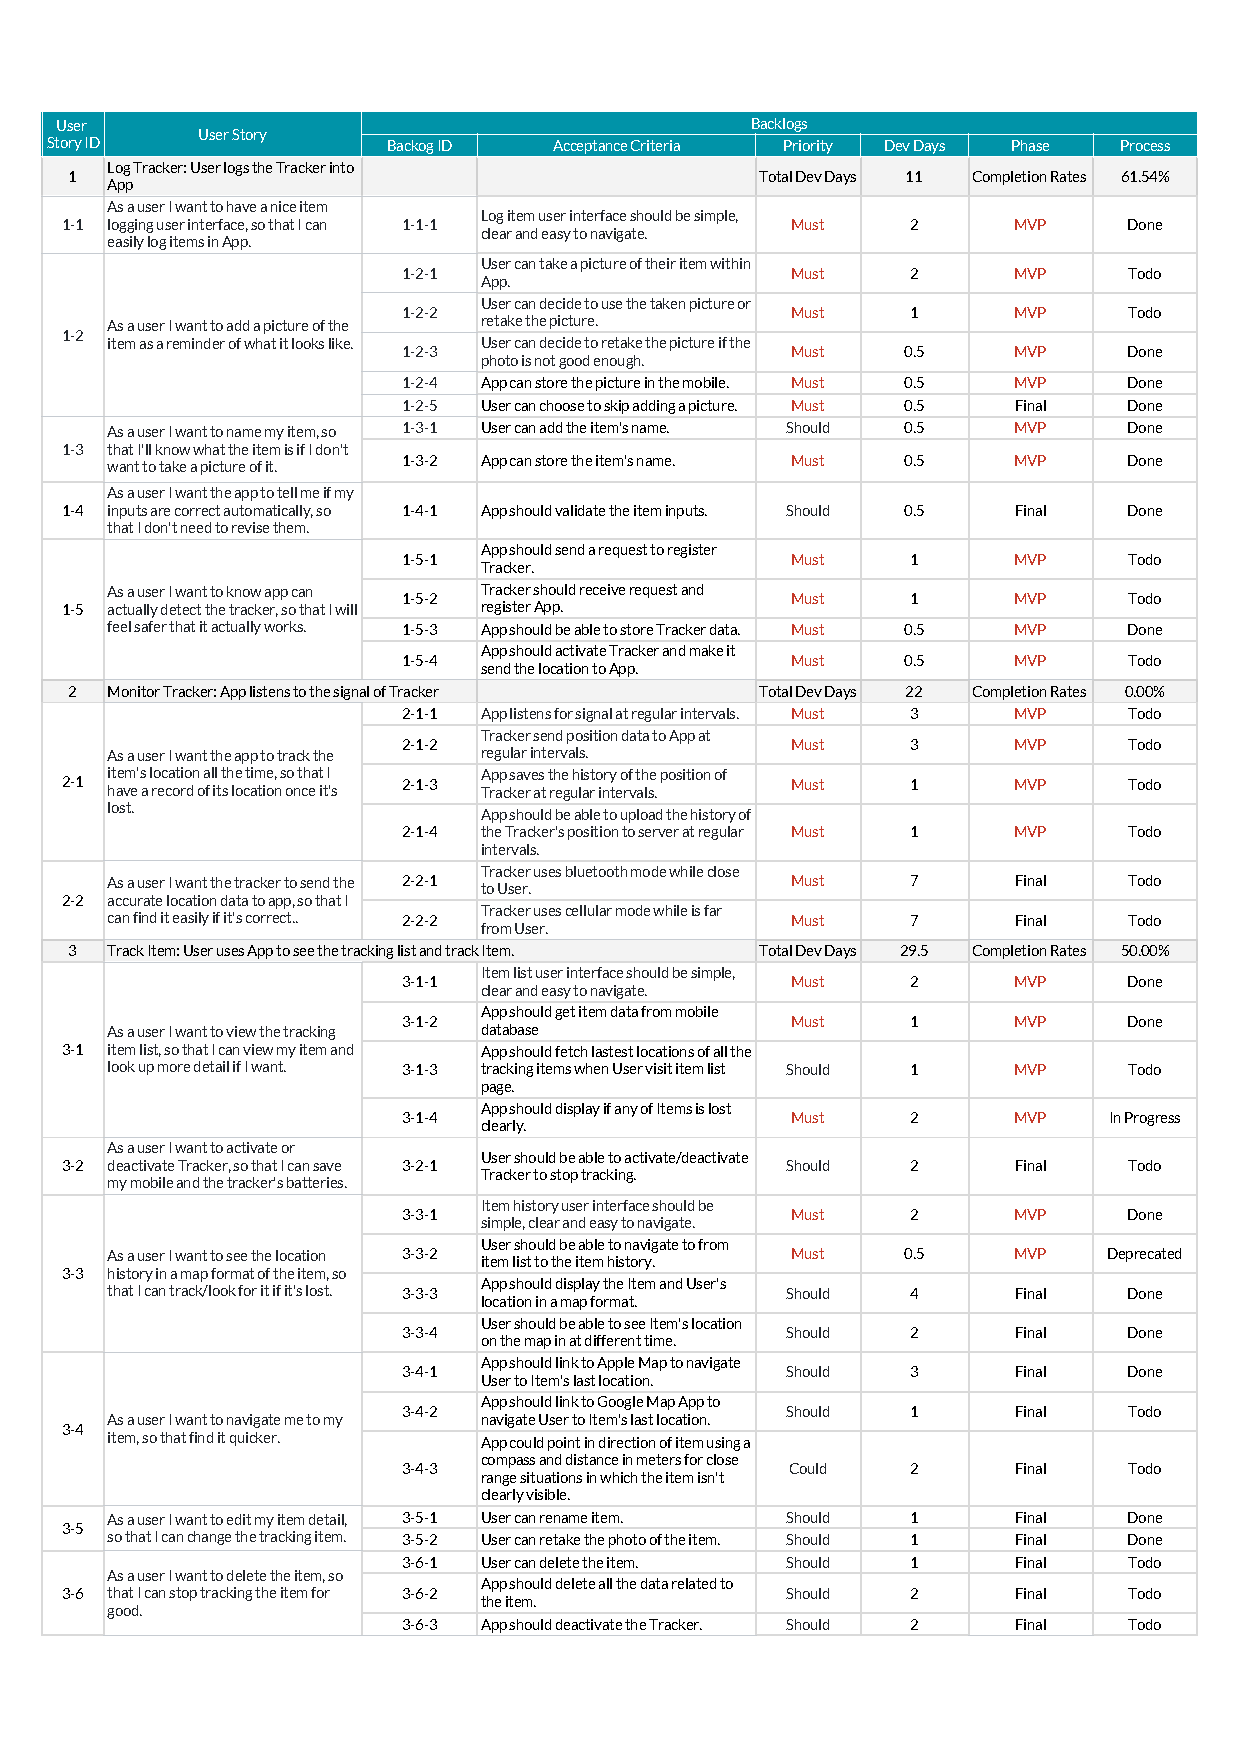
\includepdf[pages=-]{../assets/development-records-backlogs.pdf}
          
        \subsection{Architecture Decision Records}\label{appendix:Architecture Decision Records}
          \subsubsection{Mobile Development}
            \begin{table}[H]
              \centering
                \begin{tabularx}{\textwidth}{l X}
                  \hline
                  Column & Description  \\ \hline
                  Title & Which mobile OS to work on the mobile application. \\ 
                  Context & ....  \\ 
                  Decision & ...  \\ 
                  Status & ... \\ 
                  Consequences & ... \\                  
                  \hline
                \end{tabularx}
                \caption[Table caption text]{ADR Mobile Application Development}
                \label{table:ADR Mobile Application Development}
            \end{table}

          \subsubsection{iOS Development}
            \begin{table}[H]
              \centering
                \begin{tabularx}{\textwidth}{l X}
                  \hline
                  Column & Description  \\ \hline
                  Title & Which language was used for developing the iOS mobile application. \\ 
                  Context & ....  \\ 
                  Decision & ...  \\ 
                  Status & ... \\ 
                  Consequences & ... \\                  
                  \hline
                \end{tabularx}
                \caption[Table caption text]{ADR iOS Application Development}
                \label{table:ADR iOS Application Development}
            \end{table}

          \subsubsection{Android Application Development}
            \begin{table}[H]
              \centering
                \begin{tabularx}{\textwidth}{l X}
                  \hline
                  Column & Description  \\ \hline
                  Title & ... \\ 
                  Context & ....  \\ 
                  Decision & ...  \\ 
                  Status & ... \\ 
                  Consequences & ... \\                  
                  \hline
                \end{tabularx}
                \caption[Table caption text]{ADR Android Application Development}
                \label{table:ADR Android Application Development}
            \end{table}

          \subsubsection{Tracker Development}
            \begin{table}[H]
              \centering
                \begin{tabularx}{\textwidth}{l X}
                  \hline
                  Column & Description  \\ \hline
                  Title & ... \\ 
                  Context & ....  \\ 
                  Decision & ...  \\ 
                  Status & ... \\ 
                  Consequences & ... \\                  
                  \hline
                \end{tabularx}
                \caption[Table caption text]{ADR Tracker Development}
                \label{table:ADR Tracker Development}
            \end{table}

          \subsubsection{Build a customised server}
            \begin{table}[H]
              \centering
                \begin{tabularx}{\textwidth}{l X}
                  \hline
                  Column & Description  \\ \hline
                  Title & ... \\ 
                  Context & ....  \\ 
                  Decision & ...  \\ 
                  Status & ... \\ 
                  Consequences & ... \\                  
                  \hline
                \end{tabularx}
                \caption[Table caption text]{ADR Customised Server}
                \label{table:ADR Customised Server}
            \end{table}

            \subsubsection{Transfer iOS Development from Swift to React Native}
              \begin{table}[H]
                \centering
                  \begin{tabularx}{\textwidth}{l X}
                    \hline
                    Column & Description  \\ \hline
                    Title & ... \\ 
                    Context & ....  \\ 
                    Decision & ...  \\ 
                    Status & ... \\ 
                    Consequences & ... \\                  
                    \hline
                  \end{tabularx}
                  \caption[Table caption text]{ADR Transfer iOS Development from Swift to React Native}
                  \label{table:ADR Transfer iOS Development from Swift to React Native}
              \end{table}

        \subsection{Tasks Divided}
        \subsection{Progress Tracking Form}\label{appendix:progress-tracking-form}
          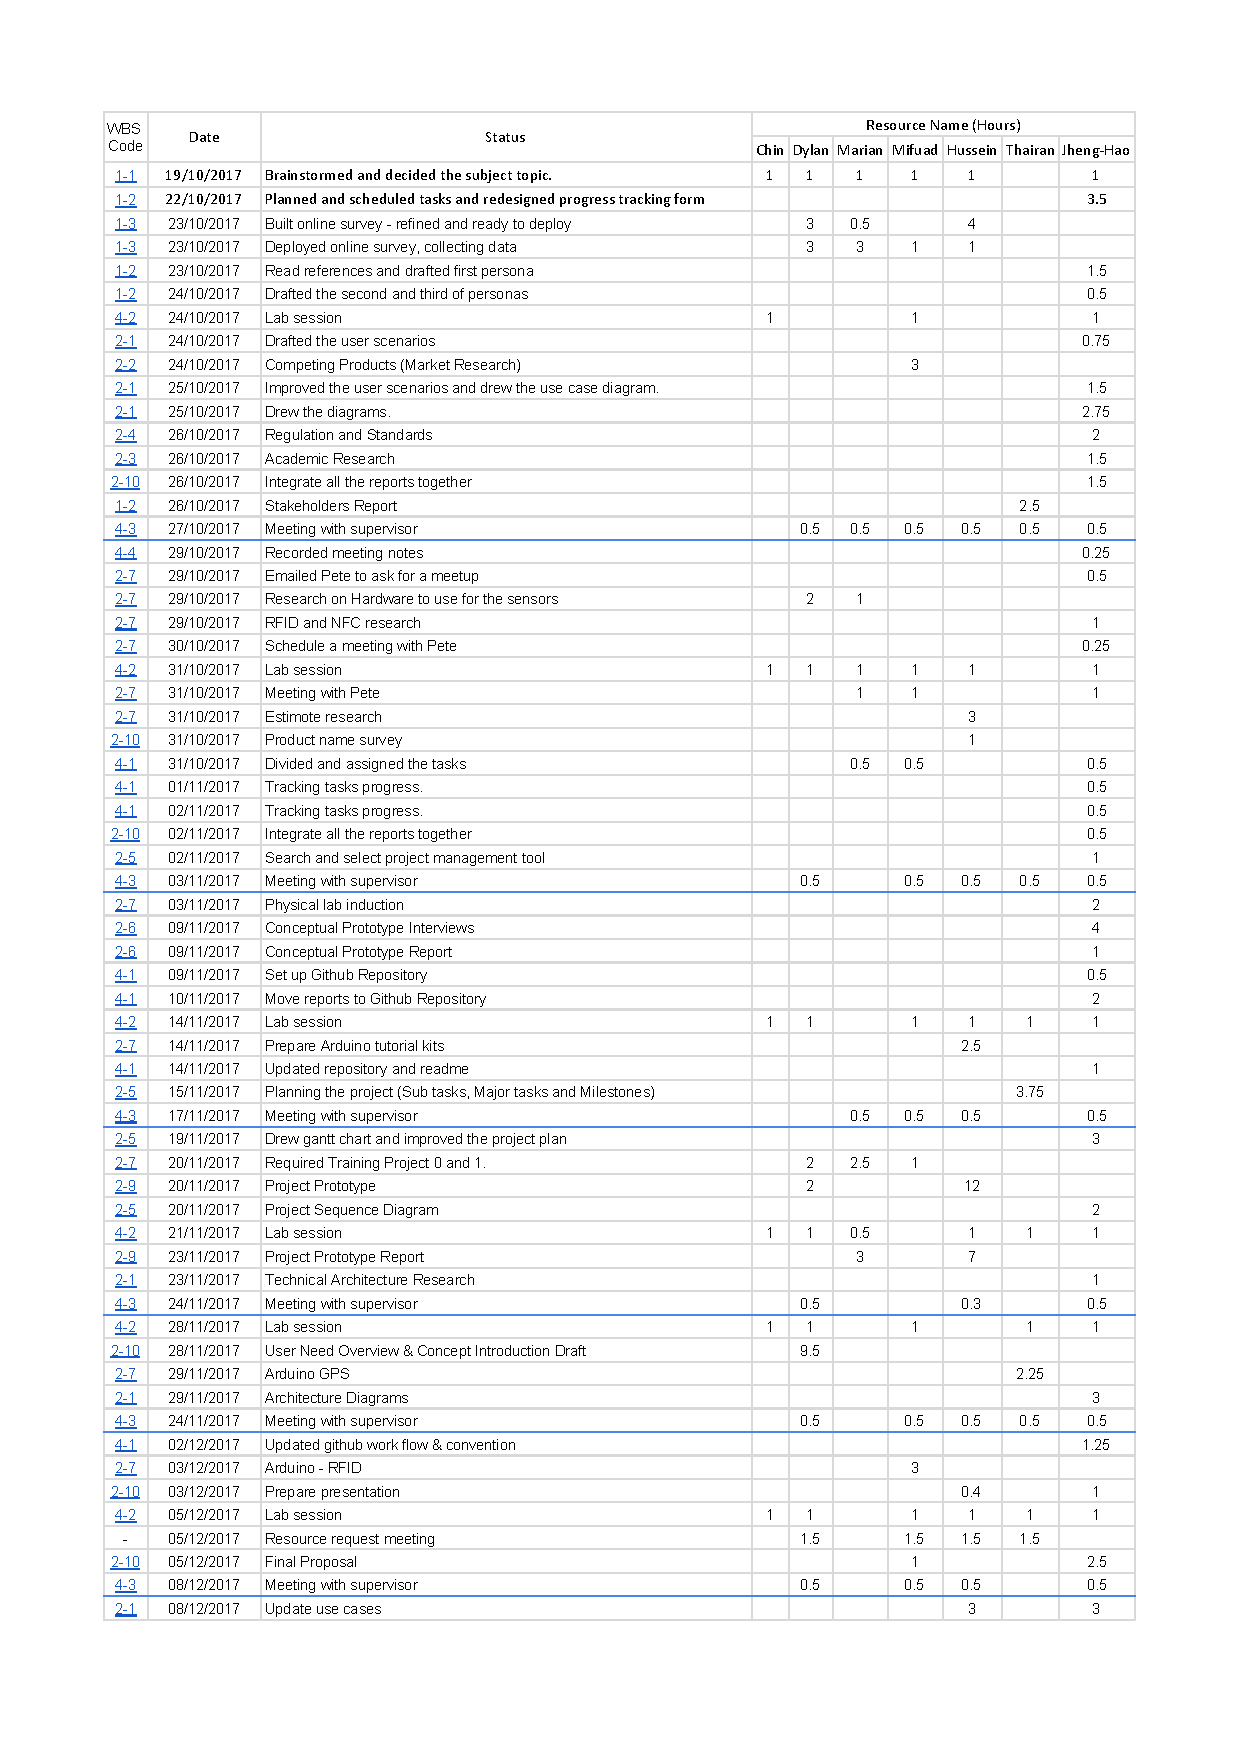
\includepdf[pages=-]{../assets/development-record-progress-tracking-form.pdf}
          
      \section{Formative Evaluation}
        \subsection{consent Form}\label{appendix:consent-form}
          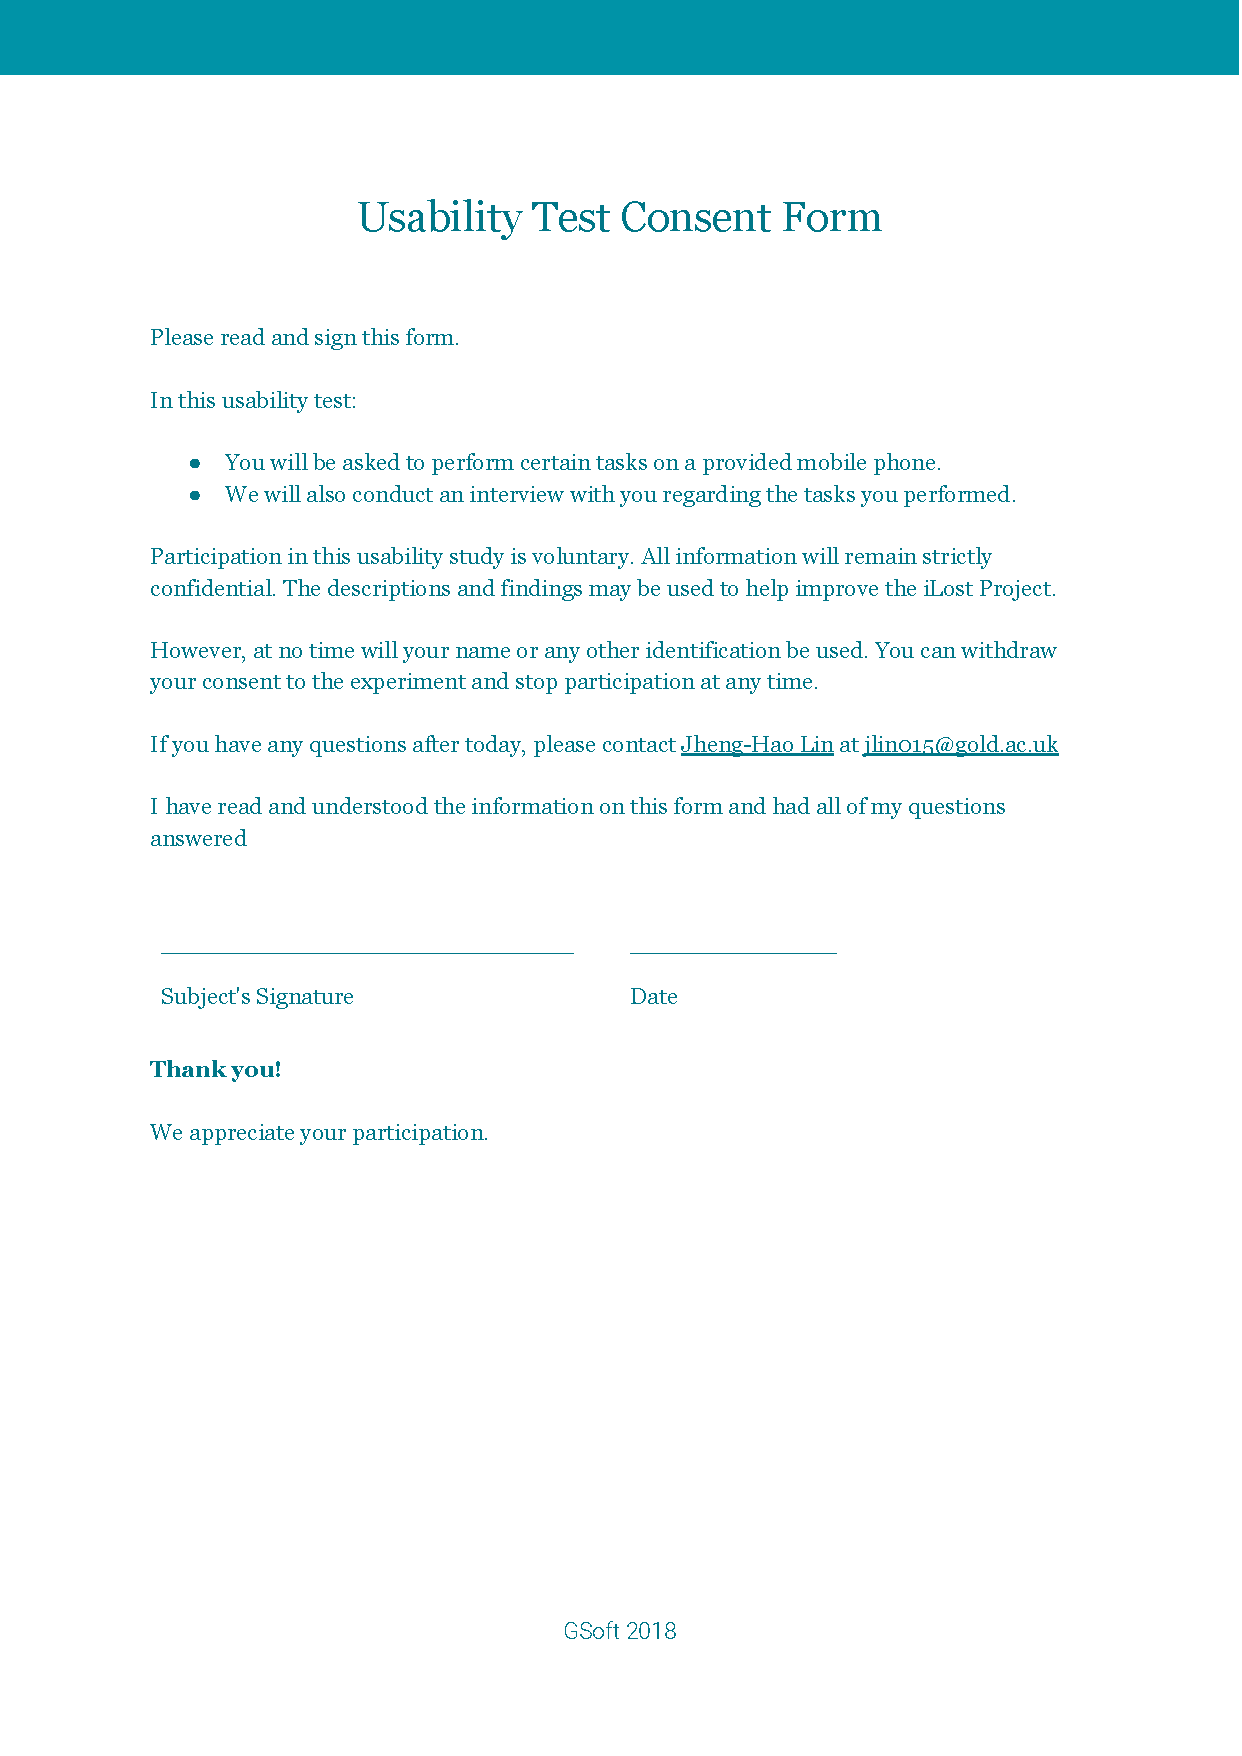
\includepdf[pages=-]{../assets/usability-test-consent-form-example.pdf}
          
      \section{Design and Implementation}
        
      \section{Quality Assurance}
        \subsection{Black-box Test Cases}\label{appendix:black-box-test-cases}
        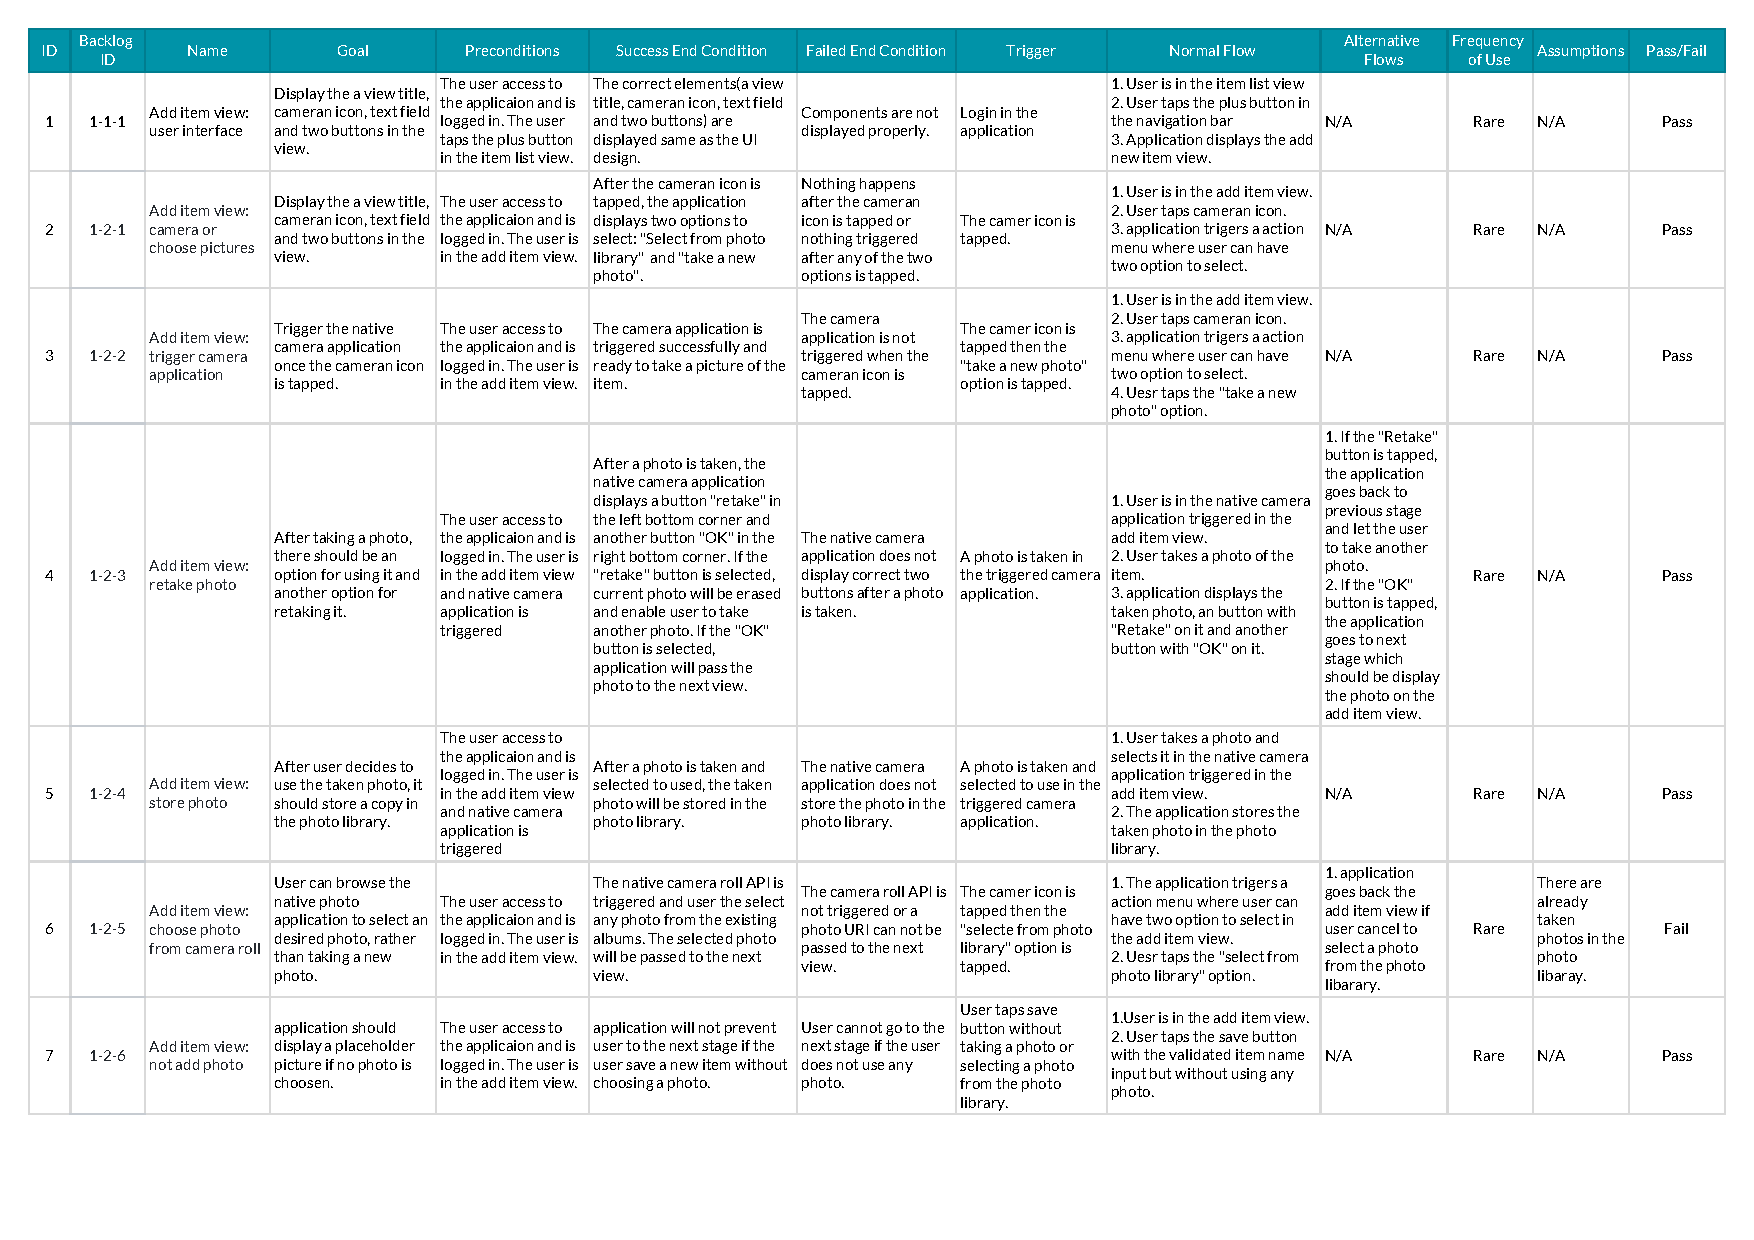
\includepdf[pages=-, angle=90]{../assets/black-box-test-cases.pdf}
    \end{appendices}

  \end{document}


